\chapter{Integración compleja}

\section{Definición de integración}

Con el objetivo de introducir los integrales de $f(z)$, consideremos primero derivadas e integrales de funciones complejas de una variable real $t$: $f: [a,b] \subset \mathbb{R} \longrightarrow \mathbb{C}$ de la forma
$$f(t) = u(t) + i v(t).$$

\begin{defi}
Se define  para la función $f$ descrita:
$$\int_a^b f(t) \,dt = \int_a^b u(t) \,dt + i \int_a^b v(t) \,dt$$

cuando las integrales individuales de la derecha existan.
\end{defi}

De forma similar se definen las integrales impropias de $f(t)$ sobre intervalos no acotados.
\\

\textbf{Observación:} Si $u$ y $v$ son funciones a valores reales continuas excepto para un número finito de puntos de $[a,b]$ y en estos puntos de discontinuidad, existen los límites laterales, podemos asegurar que ambas funciones son integrables.

Notemos que 
\begin{align*}
Re\left(  \int_a^b f(t) \,dt \right) &= \int_a^b Re[f(t)] \,dt, \\
Im\left(  \int_a^b f(t) \,dt \right) &= \int_a^b Im[f(t)] \,dt.
\end{align*}

Además, el teorema fundamental del Cálculo sobre primitivas puede extenderse a este tipo de integrales. Concretamente, supongamos que la función
$$f(t) = u(t) + i v(t)$$

es continua en el intervalo $[a,b]$, entonces existe $F(t) = U(t) + i V(t)$ tal que $F'(t) = U'(t) + i V'(t) = f(t)$, luego $U'(t) = u(t)$ y $V'(t) = v(t)$. Por lo tanto, en vista de la definición,
$$\int_a^b f(t) \,dt = U(t)|_a^b + i V(t)|_a^b = [U(b) + iV(b)] - [U(a) + iV(a)].$$

Ésto es,
$$\int_a^b f(t) \,dt = F(t) |_a^b = F(b) - F(a).$$

\begin{propo}[Propiedades de la integral]
Sean $f, g: [a,b] \longrightarrow \mathbb{C}$ integrables, se verifica que 

\begin{enumerate}

\item $\int_a^b f(t) + g(t) \,dt = \int_a^b f(t) \,dt + \int_a^b g(t) \,dt$.

\item $\int_a^b c f(t) \,dt = c \int_a^b f(t) \,dt$, para $c \in \mathbb{C}$.

\item $\int_a^b f(t) \,dt = \int_a^c f(t) \,dt + \int_c^b f(t) \,dt$, con $a \leq c \leq b$.

\item $\left| \int_a^b f(t) \,dt \right| \leq \int_a^b |f(t)| \,dt$.
\end{enumerate}
\end{propo}

\begin{proof}
Las propiedades 1., 2. y 3. son directas del Cálculo integral real.

Para 4., supongamos que 
$$\int_a^b f(t) \,dt \in \mathbb{C}-\{0\}.$$

Luego, en términos polares, tenemos que
$$r_0 e^{i\theta} = \int_a^b f(t) \,dt ~\Leftrightarrow~ r_0 = e^{-i\theta} \int_a^b f(t) \,dt ~\Leftrightarrow~ r_0 = \int_a^b e^{-i\theta} f(t) \,dt. $$

Observemos que ambos lados son números reales. Entonces, por propiedad de monotonía de las integrales del Cálculo integral real,
$$r_0 = \int_a^b Re \left( e^{-i\theta} f(t)\right) \,dt \leq \int_a^b  \left|e^{-i\theta} f(t) \right| \,dt = \int_a^b |f(t)| \,dt.$$

Así, 
$$\left|\int_a^b f(t) \,dt \right| = |r_0 e^{i\theta}| = r_0 \leq \int_a^b |f(t)|\,dt.$$

Si 
$$\int_a^b f(t) \,dt = 0,$$

la desigualdad se cumple trivialmente.

\end{proof}

Con ligeras modificaciones, la discusión para la cuarta propiedad conduce a desigualdades como
$$\left|\int_a^{\infty} f(t) \,dt \right| \leq \int_a^{\infty} |f(t)| \,dt$$

supuesto que existan ambas integrales impropias.

\section{Curvas en el plano complejo}

\begin{defi}
Una \textbf{curva} compleja es cualquier función continua
$$\gamma: [a,b] \longrightarrow \mathbb{C}.$$
\end{defi}

\begin{figure}[H]
    \centering
    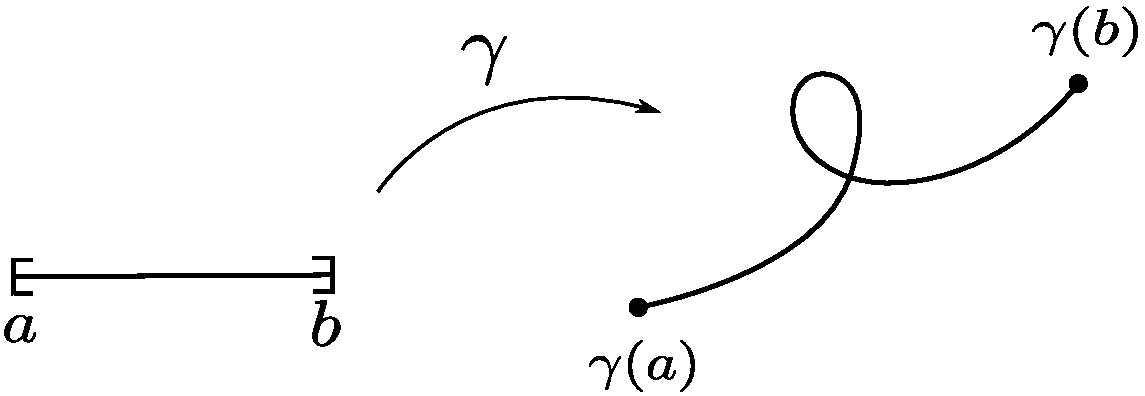
\includegraphics[scale = 0.5]{Figuras/Curva1.pdf}
    \caption{Definición de curva.}
    \label{fig:Curva1}
\end{figure}

\begin{defi}
\ 

\begin{enumerate}
\item Una curva $\gamma$ se dice de clase $C^1$ (o suave) a trazos si existe una partición finita $a = t_0 < t_1 < \cdots < t_n = b$ tal que $\gamma$ es derivable en $]t_{i-1},t_i[$ y $\gamma'(t)$ es continua en $[t_i, t_{i+1}]$; la continuidad en $[t_i, t_{i+1}]$ significa que los límites $\lim\limits_{t \to t_i^+} \gamma'(t)$ y $\lim\limits_{t\to t_{i+1}^-} \gamma'(t)$ existen.

\begin{figure}[H]
    \centering
    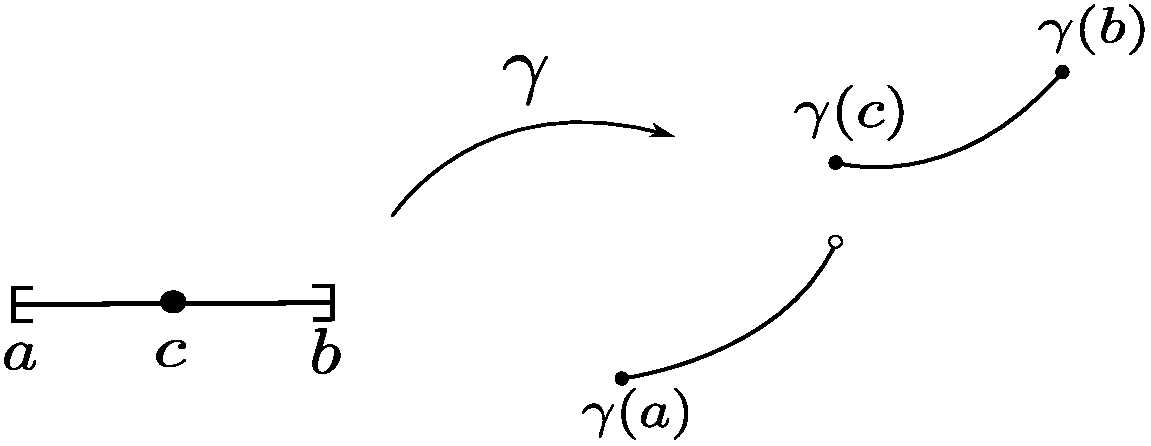
\includegraphics[scale = 0.5]{Figuras/Curva2.pdf}
    \caption{Curva suave a trazos.}
    \label{fig:Curva2}
\end{figure}

\item Una curva $\gamma : [a,b] \longrightarrow \mathbb{C}$ de clase $C^1$ se dice un \textbf{arco de Jordan} si $\gamma$ es inyectiva en $[a,b[$ (geométricamente, la curva no se cruza). Si además la curva es cerrada, la llamamos \textbf{curva de Jordan}.

\begin{figure}[H]
    \centering
    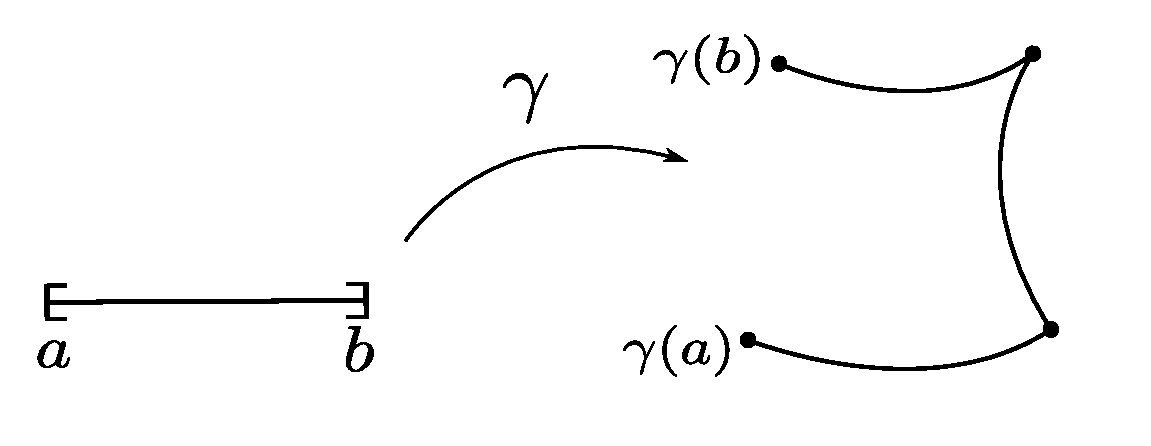
\includegraphics[scale = 0.5]{Figuras/Curva3.pdf}
    \caption{Arco de Jordan.}
    \label{fig:Curva3}
\end{figure}

\item Sea la curva $\gamma: [a,b] \longrightarrow \mathbb{C}$, se define la \textbf{curva opuesta} $- \gamma : [a,b] \longrightarrow \mathbb{C}$ como 
$$-\gamma(t) = \gamma(a+b-t).$$

\begin{figure}[H]
    \centering
    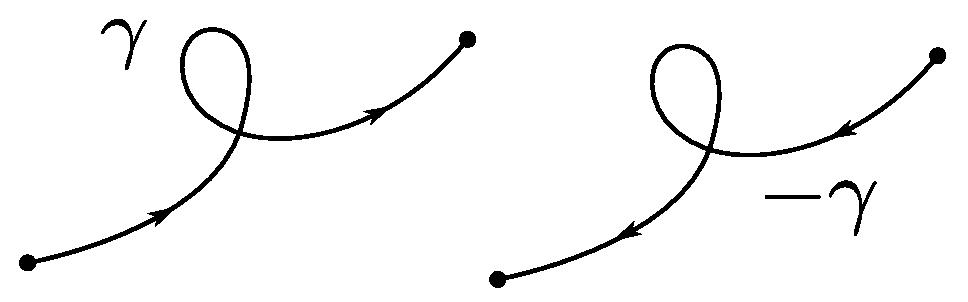
\includegraphics[scale = 0.5]{Figuras/Curva4.pdf}
    \caption{Curva opuesta.}
    \label{fig:Curva4}
\end{figure}

\end{enumerate}

\begin{ejemplo}
Una parametrización de la circunferencia centrada en el complejo $z_0$ de radio $R$ es
$$\gamma(t) = z_0 + R e^{it}, \quad t \in [0,2\pi],$$

la cual es una curva de Jordan orientada en sentido antihorario.
\end{ejemplo}

\begin{ejemplo}
Una parametrización del segmento dirigido desde el complejo $z_1$ hasta el complejo $z_2$, denotado a veces por $[z_1,z_2]$, es 
$$\gamma(t) = z_1 + t(z_2 - z_1), \quad t\in [0,1],$$

la cual es un arco de Jordan.
\end{ejemplo}

\end{defi}

\begin{defi}
 Si $\gamma_1: [a,b] \longrightarrow \mathbb{C}$ y $\gamma_2: [b,c] \longrightarrow \mathbb{C}$ son dos curvas con $\gamma_1(b) = \gamma_2(b)$, entonces se define la \textbf{unión} o \textbf{suma} de ellas $\gamma_1 + \gamma_2: [a,c] \longrightarrow \mathbb{C}$ por 
\begin{equation*}
(\gamma_1 + \gamma_2)(t) = \left\{ \begin{array}{c}
\gamma_1(t), \quad t \in [a,b] \\
\gamma_2(t), \quad t \in [b,c]
\end{array}  \right. .
\end{equation*}
\end{defi}

\begin{figure}[H]
    \centering
    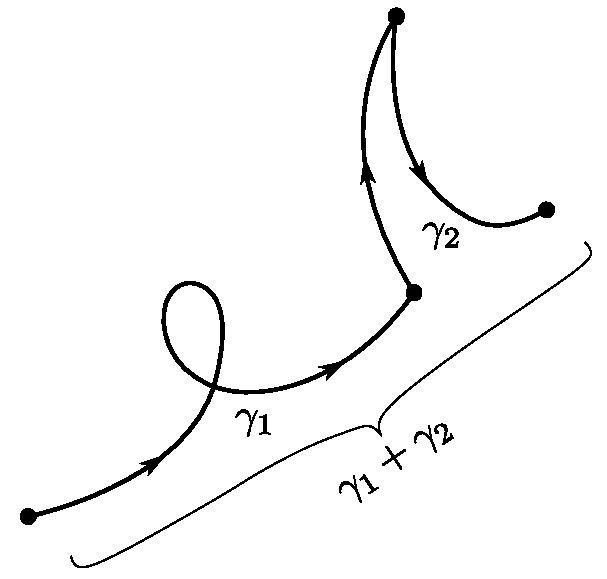
\includegraphics[scale = 0.5]{Figuras/Curva5.pdf}
    \caption{Unión de curvas.}
    \label{fig:Curva5}
\end{figure}

Claramente, si $\gamma_1$ y $\gamma_2$ son suaves por tramos, entonces también lo es $\gamma_1 + \gamma_2$.
\\

En general, sean $a, b, c,d \in \mathbb{R}$ con $a < b$ y $c < d$. Sean las curvas $\gamma_1 :[a,b] \longrightarrow \mathbb{C}$ y $\gamma_2 :[c,d] \longrightarrow \mathbb{C}$ tales que $\gamma_1(b) = \gamma_2(c)$. La suma de las curvas $\gamma_1 + \gamma_2: [a,b+(d-c)] \longrightarrow \mathbb{C}$ está definida por:
\begin{equation*}
(\gamma_1 + \gamma_2)(t) = \left\{ \begin{array}{cl}
\gamma_1(t), &\quad a \leq t \leq b \\
\gamma_2(t - (b-c)), &\quad b \leq t \leq b + (d-c)
\end{array}  \right. .
\end{equation*}

De manera natural se define la suma $\gamma_1 + \gamma_2 + \cdots + \gamma_n$ de un número finito de curvas tales que el extremo de $\gamma_j$ es el origen de $\gamma_{j-1}$ para $j = 2, \dots, n$.

\begin{defi}
Una curva (suave por tramos) $\tilde{\gamma} : [\tilde{a}, \tilde{b}] \longrightarrow \mathbb{C}$ se llama una \textbf{reparametrización} de $\gamma: [a,b] \longrightarrow \mathbb{C}$ si existe una función $\alpha: [a,b] \longrightarrow [\tilde{a}, \tilde{b}]$ de clase $C^1$ con $\alpha'(t) > 0$ para $t\in ]a,b[$, $\alpha(a) = \tilde{a}$ y $\alpha(b) = \tilde{b}$ tal que $\gamma(t) = \tilde{\gamma}(\alpha(t))$.
\end{defi}

\begin{figure}[H]
    \centering
    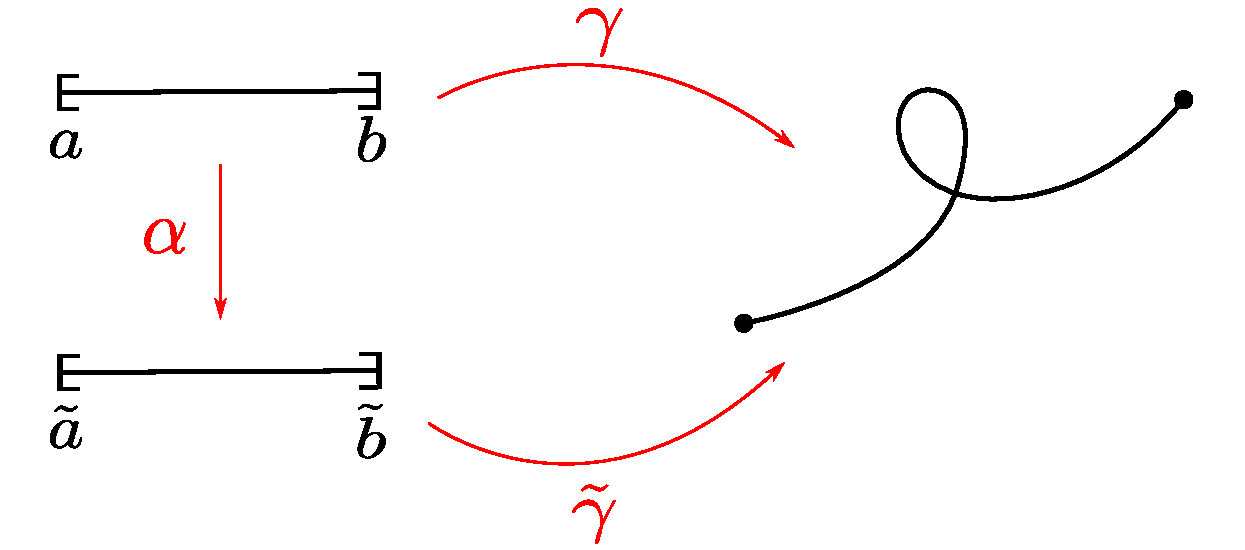
\includegraphics[scale = 0.5]{Figuras/Curva6.pdf}
    \caption{Reparametrización de una curva.}
    \label{fig:Curva6}
\end{figure}

\textbf{Observación}: Las condiciones $\alpha'(t) > 0$ (por lo que $\alpha$ es creciente), $\alpha(a) = \tilde{a}$ y $\alpha(b) = \tilde{b}$ implican que $\tilde{\gamma}$ recorre la curva en el mismo sentido que lo hace $\gamma$. La diferencia está en la velocidad en que se recorre la curva, ya que $\gamma'(t) = \tilde{\gamma}'(\alpha(t)) \cdot \alpha'(t)$. Si la función $\alpha$ fuera decreciente $(\alpha' <  0)$, la curva $\tilde{\gamma}$ sería una reparametrización de $\gamma$ recorrida en el sentido opuesto.

\section{Integral de línea}

\begin{defi}
Sea $f: A \subseteq \mathbb{C} \longrightarrow \mathbb{C}$ una función continua y sea $\gamma :[a,b] \longrightarrow \mathbb{C}$ una curva suave a trazos con $\gamma([a,b]) \subset A$ (la curva está contenida en $A$). Entonces,
$$\int_{\gamma} f  = \int_{\gamma} f(z)\, dz := \sum_{i=1}^n \int_{t_{i-1}}^{t_i} f(\gamma(t)) \gamma'(t) \,dt$$

se llama \textbf{integral de $f$ a lo largo de $\gamma$}.
\end{defi}

\textbf{Observación:} Si 
$$f(z) = u(x,y) + iv(x,y); ~ \gamma(t) = x(t) + iy(t); ~ \gamma'(t) = x'(t) + i y'(t),$$

entonces
\begin{align*}
f(\gamma(t)) \gamma'(t) &= [u(x(t), y(t)) + i v(x(t), y(t))] \cdot [x'(t) + i y'(t)] \\
&= u x' - v y' + i(uy'+vx').
\end{align*}

Así, 
\begin{equation*}
\int_{\gamma} f = \sum_{i=1}^n \int_{t_{i-1}}^{t_i} u x' - v y' + i(uy'+vx')\,dt  
= \sum_{i=1}^n \int_{t_{i-1}}^{t_i} (u x' - v y') \,dt + i \sum_{i=1}^n \int_{t_{i-1}}^{t_i} (uy'+vx') \,dt. 
\end{equation*}

Como $x'(t) dt = dx$ y $y'(t) dt = dy$, denotaremos esto último de la siguiente forma:
$$\int_{\gamma} f = \int_{\gamma} udx - vdy + i \int_{\gamma} vdx + udy.$$

\begin{teorema} \label{PropiedadesILinea}
Para funciones continuas $f,g$ y curvas suaves a trazos, $\gamma, \gamma_1, \gamma_2$, tenemos:

\begin{itemize}
\item $$\int_{\gamma} (c_1 f + c_2 g) = c_1 \int_{\gamma} f + c_2 \int_{\gamma} g, \quad c_1,c_2 \in \mathbb{C}.$$

\item $$\int_{-\gamma} f = - \int_{\gamma} f. $$

\item $$\int_{\gamma_1 + \gamma_2} f = \int_{\gamma_1} f + \int_{\gamma_2} f.$$
\end{itemize}
\end{teorema}

\begin{proof}
Ver apuntes de Cálculo III.
\end{proof}

\begin{teorema} \label{IntegralRepara}
Sea $f: A \subseteq \mathbb{C} \longrightarrow \mathbb{C}$ una función continua y sea $\gamma: [a,b] \longrightarrow \mathbb{C}$ una curva suave a tramos con $\gamma([a,b]) \subset A$ y $\tilde{\gamma}$ una reparametrización de $\gamma$. Entonces,
$$\int_{\gamma} f =  \int_{\tilde{\gamma}} f.$$

\end{teorema}

\begin{proof}
Sin pérdida de generalidad, podemos asumir que $\gamma$ es de clase $C^1$ en todo $[a,b]$.
$$\int_{\gamma} f = \int_a^b f(\gamma(t)) \gamma'(t)\,dt.$$

Ahora, como $\tilde{\gamma}$ es una reparametrización de $\gamma$ existe una función $\alpha: [a,b] \longrightarrow [\tilde{a}, \tilde{b}]$ de clase $C^1$ con $\alpha'(t) > 0$ para $t\in ]a,b[$, $\alpha(a) = \tilde{a}$ y $\alpha(b) = \tilde{b}$ tal que 
$$\gamma(t) = \tilde{\gamma}(\alpha(t)) ~\Rightarrow~ \gamma'(t) = \tilde{\gamma}'(\alpha(t)) \alpha'(t).$$

Luego, 
\begin{align*}
\int_{\gamma} f &= \int_a^b f(\tilde{\gamma}(\alpha(t))) \tilde{\gamma}'(\alpha(t)) \alpha'(t) \,dt \\
&= \int_{\tilde{a}}^{\tilde{b}} f(\tilde{\gamma}(s)) \tilde{\gamma}'(s)\,ds \qquad (s = \alpha(t) \Rightarrow ds = \alpha'(t) dt) \\
&= \int_{\tilde{\gamma}} f.
\end{align*}
\end{proof}

\begin{ejemplo}
Calcular
$$\int_C \overline{z} \,dz$$

donde $C$ es la mitad derecha de la circunferencia $|z| = 2$ orientada en sentido antihorario.
\\

\textbf{Solución:} Una parametrización de $C$ es
$$\gamma: [- \pi/2, \pi/2] \longrightarrow \mathbb{C}, \gamma(t) = 2 e^{i t}.$$

\begin{figure}[H]
    \centering
    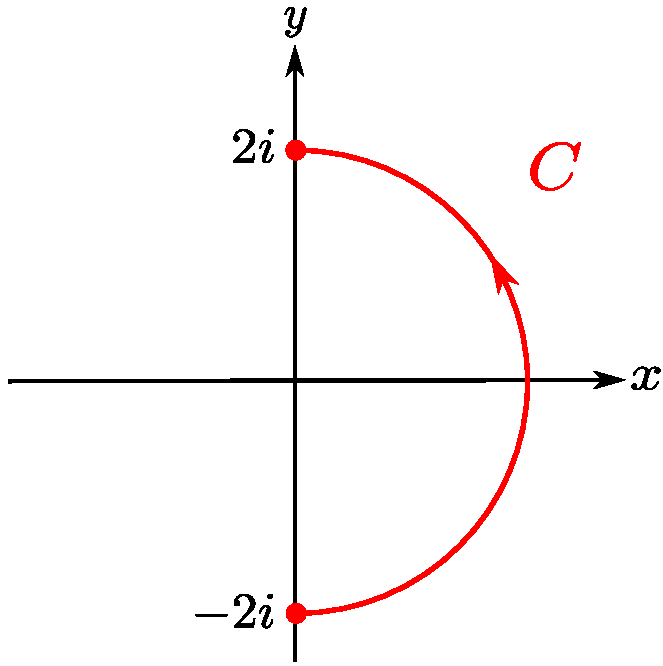
\includegraphics[scale = 0.5]{Figuras/Integral1.pdf}
    \caption{Mitad derecha de la circunferencia $|z| = 2$.}
    \label{fig:IntegralLinea1}
\end{figure}

\vspace{-0.4cm}

Tenemos que $C$ es suave con 
$$\gamma'(t) = 2 i e^{i t}.$$

Luego, por definición, 
\begin{equation*}
\int_C \overline{z} \,dz = \int_{- \pi/2}^{\pi/2} 2 e^{-it} 2 i e^{i t} \,dt = 4i \int_{-\pi/2}^{\pi/2}\, dt = 4 \pi i.
\end{equation*}
\end{ejemplo}

\begin{ejemplo}
Calcular
$$\int_C f(z) \,dz$$

donde $f(z) = y - x - i3x^2$ y $C$ es la unión del segmento que va desde 0 a $i$ y del segmento desde $i$ a $1+i$.
\\

\textbf{Solución}:  Sea $C_1$ el segmento desde $0$ a $i$ y $C_2$ el segmento desde $i$ a $1+i$, tenemos que
$$\int_C f(z) \,dz = \int_{C_1} f(z) \,dz + \int_{C_2} f(z) \,dz.$$

\begin{figure}[H]
    \centering
    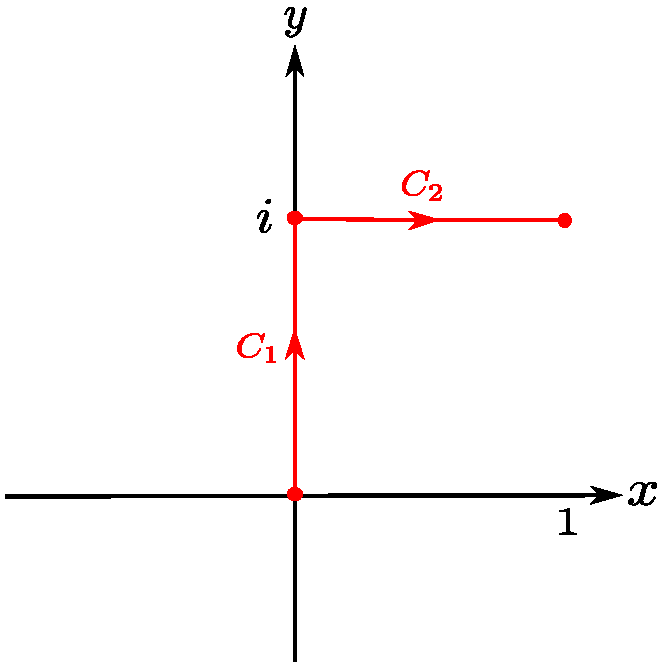
\includegraphics[scale = 0.5]{Figuras/Integral2.pdf}
    \caption{Unión del segmento desde $0$ a $i$ y del segmento $i$ a $1+i$.}
    \label{fig:IntegralLinea2}
\end{figure}

Las parametrizaciones para $C_1$ y $C_2$ son, respectivamente,
\begin{align*}
\gamma_1: [0,1] \longrightarrow \mathbb{C}, \gamma_1(t) &= it \\
\gamma_2: [0,1] \longrightarrow \mathbb{C}, \gamma_2(t) &= t + i
\end{align*}

Entonces, $C = C_1 + C_2$ es suave por trazos con 
$$\gamma_1\,'(t) = i ~~\mbox{y}~~ \gamma_2\,'(t) = 1.$$

Por definición,
\begin{align*}
\int_{C_1} f &= \int_0^1 t i \,dt = \left. i \frac{t^2}{2} \right|_0^1 = \frac{i}{2}, \\
\int_{C_2} f &= \int_0^1 (1-t-i3t^2) 1 \,dt = \left. t - \frac{t^2}{2} - it^3 \right|_0^1 = \frac{1}{2} - i.
\end{align*}

Por lo tanto, 
$$\int_C f(z) \,dz = \frac{i}{2} + \frac{1}{2} - i = \frac{1}{2} - \frac{i}{2}.$$
\end{ejemplo}

De Cálculo III, sabemos que si $\gamma$ es un arco de Jordan, ésta es rectificable y su longitud viene dada por 
$$l(\gamma) = \int_a^b |\gamma'(t)| \,dt = \int_a^b \sqrt{[x'(t)]^2 + [y'(t)]^2} \,dt$$

y que es independiente de la parametrización de $\gamma$.

\begin{teorema} \label{CotaIntegral}
Sea $f: A \subseteq \mathbb{C} \longrightarrow \mathbb{C}$ una función  continua y sea $\gamma: [a,b] \longrightarrow \mathbb{C}$ una curva suave por tramos con $\gamma([a,b]) \subset A$. Si existe una constante $M > 0$ tal que $|f(z)| \leq M$ para todo los puntos $z$ traza de $\gamma$\footnote{ Que $z$ sea parte de la traza de $\gamma$ significa que existe $t \in [a,b]$ tal que $z = \gamma(t)$.  }, entonces
$$\left|\int_{\gamma} f \right| \leq M l(\gamma).$$

Más general, tenemos
$$\left|\int_{\gamma} f \right| \leq \int_{\gamma} |f| \,|dz|$$

donde la última integral se define como 
$$\int_{\gamma} |f| |dz| := \int_a^b |f(\gamma(t))|\, |\gamma'(t)| \,dt.$$
\end{teorema}

\begin{proof}

Supongamos, sin pérdida de generalidad, que la curva $\gamma$ es suave. Entonces, podemos escribir
\begin{align*}
\left| \int_{\gamma} f \right| &= \left| \int_a^b f(\gamma(t)) \gamma'(t) \,dt \right| \\
&\leq \int_a^b |f(\gamma(t)) \gamma'(t)| \,dt = \int_a^b |f(\gamma(t))| \, |\gamma'(t)| \,dt.
\end{align*}

Como $|f(\gamma(t))| \leq M$ para todo $t \in [a,b]$, la expresión nos queda
\begin{equation*}
\int_a^b |f(\gamma(t))| \, |\gamma'(t)| \,dt \leq M \int_a^b |\gamma'(t)| \,dt = M l(\gamma).
\end{equation*}

\end{proof}

\begin{ejemplo}
Sea $\gamma$ la mitad de la circunferencia unitaria descrita contraria a las agujas del reloj. Mostrar que 
$$\left| \int_{\gamma} \frac{e^z}{z}\right| \leq \pi e.$$

\textbf{Solución}: Notemos que 
$$l(\gamma) = \int_0^{\pi} |\gamma'(t)| \,dt = \pi$$

pues $\gamma(t) = e^{it}, 0 \leq t \leq \pi$ y $\gamma'(t)= i e^{it}$. 

Ahora, para $z$ en la semi-circunferencia, descrita por $\gamma$, existe $t \in [0,\pi]$ tal que $z = e^{it} = \cos t + i \sin t$ y 
$$\left| \frac{e^z}{z}\right| = \frac{|e^{\cos t} e^{i\sin t}|}{|e^{it}|} = \frac{e^{\cos t}}{1} \leq e = M.$$

Así,
$$\left| \int_{\gamma} \frac{e^z}{z}\right| \leq \pi e.$$
\end{ejemplo}

\section{Independencia del camino}

El siguiente teorema es análogo al Teorema Fundamental del Cálculo:

\begin{teorema} \label{TFClinea}
Sea $f: A \subseteq \mathbb{C} \longrightarrow \mathbb{C}$ una función continua tal que $f = F\,'$ para alguna función analítica $F: A \longrightarrow \mathbb{C}$. Sea $\gamma: [a,b] \longrightarrow \mathbb{C}$ una curva suave a trazos con $\gamma([a,b]) \subseteq A$ y que une los puntos $\gamma(a) = z_1$ y $\gamma(b) = z_2$. Entonces,
$$\int_{\gamma} f = F(z_2) - F(z_1).$$

En particular, si $z_1 = z_2$ (es decir, una curva cerrada), entonces
$$\int_{\gamma} f = 0.$$
\end{teorema}

\begin{proof}
Por regla de la cadena, tenemos que 
$$(F \circ \gamma)'(t) = F\,'(\gamma(t)) \gamma\,'(t) = f(\gamma(t)) \gamma\,'(t).$$

Así,
\begin{align*}
    \int_{\gamma} f = \int_a^b f(\gamma(t)) \gamma\,'(t) \,dt &= \int_a^b (F \circ \gamma)'(t) \,dt \\
    &= F(\gamma(b)) - F(\gamma(a))\\
    &= F(z_2) - F(z_1).
\end{align*} 
\end{proof}

\begin{defi}
Toda función $F$ tal que $f = F\,'$ para todo $z$ en un dominio $D$, se llama \textbf{primitiva} o \textbf{antiderivada} de $f$
\end{defi}

\begin{teorema}[Independencia del camino]  \label{TFC2}
Sea $f(z)$ una función continua en un abierto conexo $D$ (una región). Si cualquiera de estas afirmaciones es verdadera, lo son también las demás:
\begin{itemize}
    \item[a)] $f$ tiene una primitiva $F$ en $D$;
    
    \item[b)] las integrales de $f$ a lo largo de curvas contenidas en $D$ que unen puntos fijos $z_1$ y $z_2$ tienen todas el mismo valor;
    
    \item[c)] las integrales de $f$ a lo largo de cualquier curva cerrada contenida en $D$ es cero.
\end{itemize}
\end{teorema}

\begin{proof}
Para demostrar el teorema es suficiente probar las equivalencias entre a) y b); b) y c).

\begin{itemize}
    \item $a) \Rightarrow b)$: Directo del teorema \ref{TFClinea}.
    
    \item $b) \Rightarrow a)$: Necesitamos mostrar que si la integral es independiente de la curva, entonces $f$ tiene una antiderivada $F$. Fijamos $z_0 \in D$ y definimos
    $$F(z) = \int_{\gamma(z_0,z)} f(\xi) \,d\xi,$$
    
    donde $\gamma(z_0,z)$ es una curva que une $z_0$ y $z$, ver figura \ref{fig:IntegralLinea1}. Tal curva existe porque $D$ es conexo. Esto define una función $F$ en $D$ sin ambigüedad alguna, pues b) nos dice que el valor de $F(z)$ depende de $z$ y no de la trayectoria elegida, en tanto se encuentre en $D$. 
    
    Sea $\varepsilon > 0$, como $D$ es abierto y $f$ es continua en $z$, existe un número $\delta > 0$ tal que la bola abierta $B(z, \delta) \subseteq D$ y $|f(\xi) - f(z)| < \varepsilon$ siempre que $|\xi - z| < \delta$. Si escogemos $z+w \in B(z, \delta)$ y conectamos $z$ a $z+w$ por medio de un segmento $[z,z+w]$. Entonces, todo $[z,z+w]$ descansa en $B(z,\delta)$, ver figura \ref{fig:IntegralLinea1},  y
    $$F(z+w) - F(z) = \int_{\gamma(z_0,z) + [z,z+w]} f(\xi) \,d\xi - \int_{\gamma(z_0,z)} f(\xi) \,d\xi = \int_{[z,z+w]} f(\xi) \,d\xi.$$
    
    Así, si $|(z+w)-z| = |w| < \delta$, se cumple que
    \begin{align*}
       \left|\frac{F(z+w)-F(z)}{w} - f(z)\right| &=  \frac{|F(z+w) - F(z) - w f(z)|}{|w|} \\
       &= \frac{1}{|w|} \left| \int_{[z,z+w]} f(\xi) \,d\xi -f(z) \int_{[z,z+w]} 1 \,d\xi  \right| \\
       &= \frac{1}{|w|} \left| \int_{[z,z+w]} [f(\xi) - f(z)] \,d\xi   \right| \\
       &\leq \frac{\varepsilon}{|w|}l([z,z+w]) \quad (Teorema \ref{CotaIntegral})\\
       &= \frac{\varepsilon}{|w|} |w| = \varepsilon.
    \end{align*}

Probando así que
$$\lim_{w \to 0} \frac{F(z+w)- F(z)}{w} = f(z),$$

ésto es, $F$ es derivable y $F\,' = f$.

   \begin{figure}[H]
        \centering
        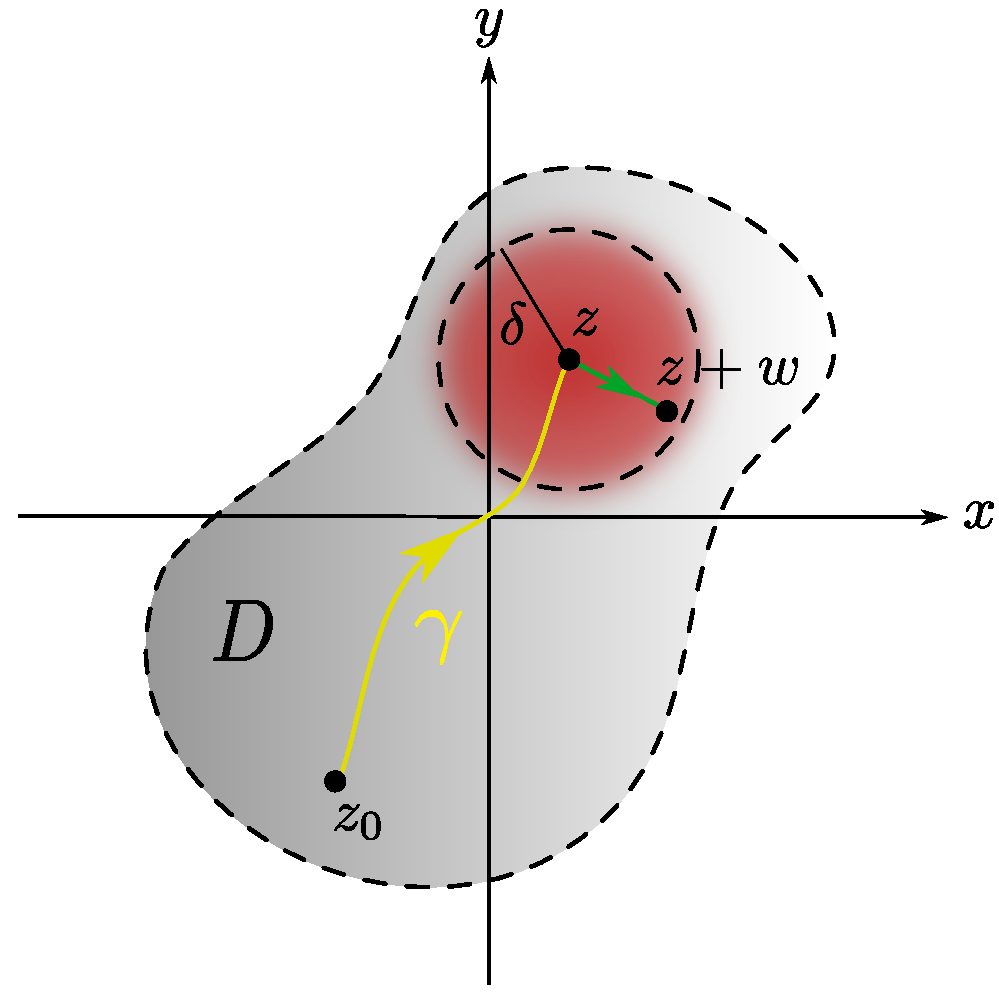
\includegraphics[scale = 0.45]{Figuras/TFCIntegralLinea1.pdf}
        \caption{Visión geométrica de la demostración.}
        \label{fig:TFC1}
    \end{figure}

\item $b) \Rightarrow c)$: Es directo de usar a).

\item $c) \Rightarrow a)$: Consideremos dos curvas $\gamma_1$ y $\gamma_2$ suaves por trazos que unen dos puntos $z_1$ y $z_2$ en $D$, y sea $\Gamma$ la curva cerrada que surge al unir $\gamma_1$ y $- \gamma_2$. Entonces,
$$0 = \int_{\Gamma} f(z) \,dz = \int_{\gamma_1} f(z) \,dz + \int_{-\gamma_2} f(z) = \int_{\gamma_1} f(z) \,dz - \int_{\gamma_2} f(z),$$
implicando que 
$$\int_{\gamma_1} f(z) \,dz = \int_{\gamma_2} f(z) \,dz.$$

Por lo tanto, la integral de $f$ es independiente de la curva.

 \begin{figure}[H]
        \centering
        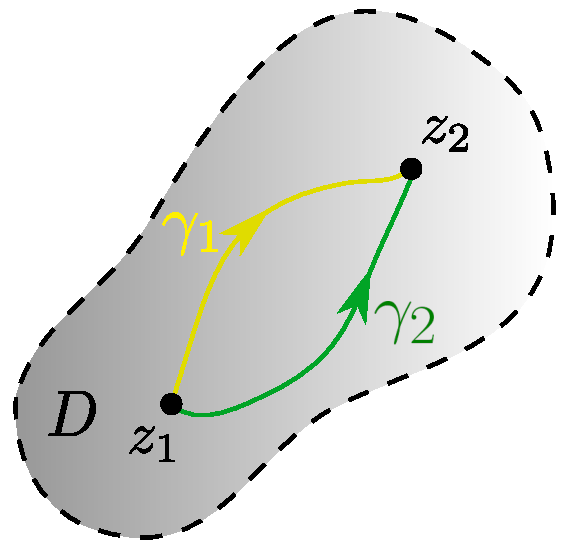
\includegraphics[scale = 0.45]{Figuras/TFCIntegralLinea2.pdf}
        \caption{Dos curvas con los mismos extremos.}
        \label{fig:TFC2}
    \end{figure}
\end{itemize}
\end{proof}

\begin{ejemplo}
Calcular
$$\int_{\gamma} e^z dz,$$

donde $\gamma(t) = e^{it}$, $0 \leq t \leq \pi.$
\\

\textbf{Solución:} La función $e^z$ es continua en todo el plano complejo, con antiderivada $e^z$. El punto inicial de $\gamma$ es $z_1 = \gamma(0) = 1$ y su punto terminal es $z_2 = \gamma(\pi) = -1$. Entonces,
$$\int_{\gamma} e^z dz = \left. e^z \right|_{1}^{-1} = e^{-1}-e^1 = - 2 \sinh(1).$$
\end{ejemplo}

\begin{ejemplo}
Evaluar 
$$\int_C \frac{1}{z} dz,$$

donde $C$ es el camino poligonal que parte de $1$ al $2+i$ y termina en $3$, ver figura \ref{fig:EjTFC1}.
\\

\textbf{Solución:} La función $1/z$ es continua en $\mathbb{C} \setminus \{0\}$. Una antiderivada de $1/z$ es $Log(z) = \ln |z| + i Arg(z)$ en la región $D = \mathbb{C}\setminus ]-\infty, 0]$. La curva $C$ yace enteramente en $D$, ver figura \ref{fig:EjTFC1}.

   \begin{figure}[H]
        \centering
        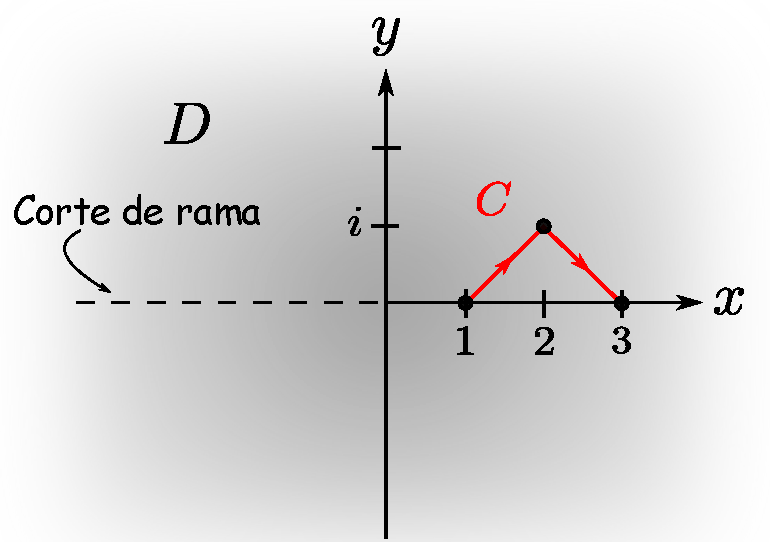
\includegraphics[scale = 0.5]{Figuras/Ejemplo_TFCIntegralLinea1.pdf}
        \caption{Camino poligonal que inicia del $1$ se va al $2+i$ y termina en $3$.}
        \label{fig:EjTFC1}
    \end{figure}
    
Así, 
$$\int_C \frac{1}{z} dz = \left. Log(z) \right|_1^3 = \ln(3).$$
\end{ejemplo}

\begin{ejemplo}
Evaluar 
$$\int_C \frac{1}{z} dz,$$

donde $C$ es el camino poligonal que parte de $-1$ al $-1+i$ y termina en $-2-2i$, ver figura \ref{fig:EjTFC2}.
\\

\textbf{Solución:} Para aplicar el teorema debemos encontrar una antiderivada de $1/z$ que sea analítica en la región que contiene a la curva $C$. En este caso, no podemos usar $Log(z)$ como antiderivada porque no es analítica en una región que contenga a $C$ (la curva pasa por el corte de ramificación). En su lugar, debemos usar otra rama del logaritmo. Sabemos que al considerar $\alpha < \arg(z) < \alpha + 2\pi$ para un cierto $\alpha \in \mathbb{R}$, se obtiene una rama de $\log(z)$ analítica. 

Tomando, por ejemplo, $\alpha = 0$, podemos escribir 
$$\log(z) \rightarrow \log_0(z) = \ln|z| + i \arg_0(z),$$

donde $0 < \arg_0(z) < 2\pi$, la cual es una antiderivada de $1/z$, analítica en la región $D = \mathbb{C}\setminus [0, +\infty[$ donde yace la curva $C$. Así,
\begin{align*}
    \int_C \frac{1}{z} dz &= \log_0(-2-2i) - \log_0(-1) \\
    &= \ln|-2-2i| + i \arg_0(-2-2i) - (\ln(1) + i \arg_0(-1)) \\
    &= \frac{1}{2} \ln(8) + i \frac{5\pi}{4} - i \pi = \frac{3}{2} \ln(2) + i\frac{\pi}{4}.
\end{align*}

\begin{figure}[H]
        \centering
        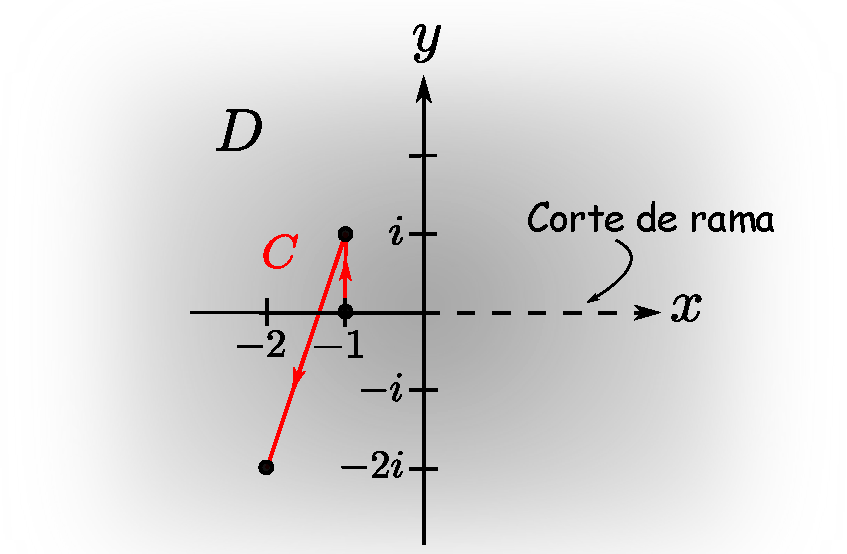
\includegraphics[scale = 0.5]{Figuras/Ejemplo_TFCIntegralLinea2.pdf}
        \caption{Camino poligonal que inicia del $-1$ se va al $-1+i$ y termina en $-2-2i$.}
        \label{fig:EjTFC2}
    \end{figure}
\end{ejemplo}

\section{Teorema de Cauchy-Goursat}

Recordemos el teorema de Green en su primera forma del Cálculo III.

\begin{teorema}[de Green primera forma]
Sea $\gamma$ una curva de Jordan con orientación positiva y sea $R$ la reunión de $C$ y de su interior. Si $\Vec{F}(x,y) = P(x,y) \hat{\imath} + Q(x,y) \hat{\jmath}$ es de clase $C^1$ en un abierto $A$ que contiene a $R$, entonces
$$\oint_{\gamma} Pdx + Qdy = \iint_R \left[ \frac{\partial Q}{\partial x} - \frac{\partial P}{\partial y}\right] \,d(x,y).$$
\end{teorema}

Este teorema permite demostrar el siguiente resultado.

\begin{teorema}[de Cauchy]
Si $f$ es analítica en todos los puntos encerrados por una curva simple cerrada $\gamma$ y $f'$ es continua en dicha región, entonces
$$\int_{\gamma} f = 0.$$
\end{teorema}

\begin{proof}
Consideremos $f(z) = u(x,y) + iv(x,y)$ una función analítica en una región $R$ que contiene el interior de la curva $\gamma$, que supondremos de orientación positiva, y su frontera. Entonces, como $f'(z) = u_x + i v_x = v_y - iu_y$  es continua, $u$ y $v$ tienen derivadas parciales continuas. De esta manera, podemos aplicar el teorema de Green en su primera forma y obtener que
\begin{align*}
    \int_{\gamma} udx - vdy &= - \iint_R (v_x + u_y) \,d(x,y), \\
    \int_{\gamma} vdx + udy &=  \iint_R (u_x - v_y) \,d(x,y).
\end{align*}

Por las ecuaciones de Cauchy-Riemann, concluimos que ambas integrales son nulas. Así,
$$\int_{\gamma} f = \int_{\gamma} udx - vdy + i \int_{\gamma} vdx + udy = 0.$$

Si la curva tiene orientación negativa, la conclusión es la misma.

\end{proof}

Goursat fue el primero en demostrar que la condición de continuidad de $f'$ se puede omitir, dando paso a la versión modificada del teorema de Cauchy, conocida como el \textbf{teorema de Cauchy-Goursat} cuya demostración se escapa del curso.

\begin{teorema}[de Cauchy-Goursat]
Si $f$ es analítica en todos los puntos encerrados por una curva simple cerrada $\gamma$, entonces
$$\int_{\gamma} f = 0.$$
\end{teorema}

\textbf{Observación:} Consideremos la función $f(z) = \frac{1}{z}$ y supongamos que $\gamma$ es la circunferencia centrada en el origen de radio 1. $f$ es analítica en todo punto excepto en $z = 0$.

Por otro lado,
\begin{equation}
 \int_{\gamma} \frac{1}{z} = \int_0^{2\pi} \frac{1}{e^{it}} i e^{it} dt = \int_0^{2\pi} i  dt = 2\pi i \neq 0. \label{PreTIC}  
\end{equation}

Esto nos dice que, la hipótesis de analiticidad en todo el interior no puede ser debilitada.

\section{Dominios simplemente conexos y múltiplemente conexos}

\begin{defi}
Sea $D$ un abierto conexo del plano complejo. Se dice que $D$ es una \textbf{región simplemente conexa} si toda curva simple cerrada en $D$ encierra sólo puntos de $D$, en otras palabras, $D$ no tiene agujeros. Los conjuntos que no son simplemente conexos se llaman \textbf{múltiplemente conexos}.
\end{defi}

\begin{figure}[H]
    \centering
    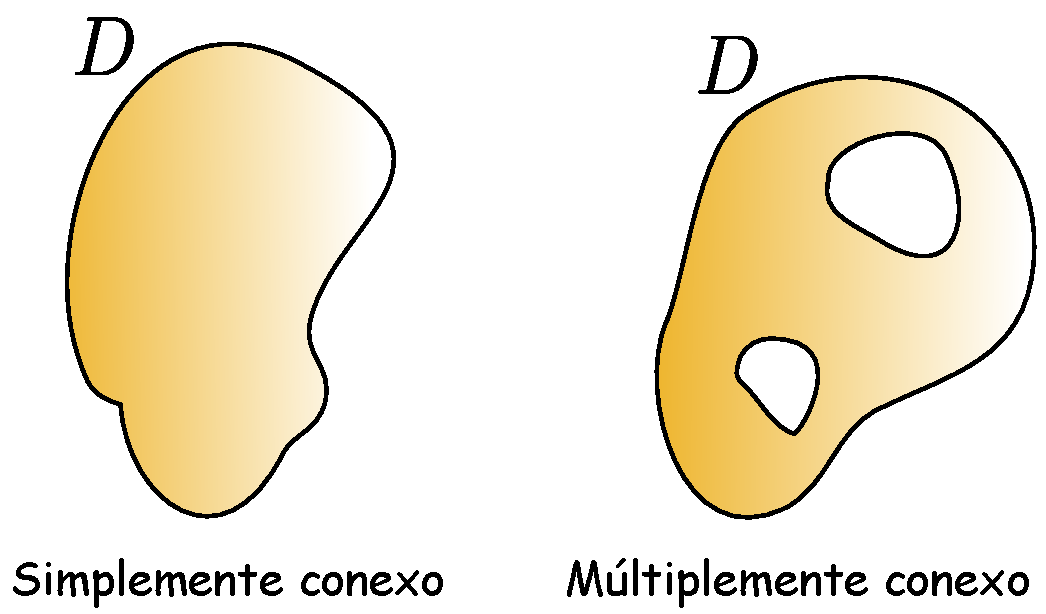
\includegraphics[scale = 0.5]{Figuras/SimplementeConexo.pdf}
    \caption{Dominios simplemente conexo y múltiplemente conexo.}
    \label{fig:SimConexo}
\end{figure}

El teorema de Cauchy-Goursat admite la siguiente extensión relativa a dominios simplemente conexos.

\begin{teorema} \label{CG-SC}
Si una función $f$ es analítica en un dominio simplemente conexo $D$, entonces 
$$\int_{\gamma} f(z) \,dz = 0$$

para toda curva cerrada $\gamma$ contenida en $D$.
\end{teorema}

\begin{proof}
Consulte la sección 3.6 de \cite{Asmar}.
\end{proof}

\begin{corolario}
Una función $f$ que es analítica sobre un dominio simplemente conexo $D$ tiene primitiva en $D$ y la integral es independiente de la curva que une a dos puntos $z_1,z_2 \in D$.
\end{corolario}

\begin{proof}
Consecuencia inmediata del teorema \ref{CG-SC}, a causa del teorema \ref{TFC2}.
\end{proof}

El teorema de Cauchy-Goursat se puede extender a dominos múltiplemente conexos

\begin{teorema} \label{CGMultiConexo}
Sea $\gamma$ una curva simple cerrada y sean $\gamma_1, \gamma_2, \dots, \gamma_n$ curvas simples cerradas que se encuentran al interior de $\gamma$ y éstas no se cortan. Sea $R$ la región de todo los puntos al interior de $\gamma$ y al exterior de $\gamma_j$, $j = 1,2, \dots, n$. Entonces, $f$ analítica en $R$ implica que 
$$\int_{\gamma} f = \sum_{j=1}^n \int_{\gamma_j} f,$$

donde se asume que las orientaciones de las curvas son positivas.
\end{teorema}

\begin{proof}
Fijemos un punto $z_0$ en la curva $\gamma$. Por medio de un segmento $L_1$ unimos $z_0$ a un punto $w_1$ en $\gamma_1$. Escogemos $z_1$ en $\gamma_1$ y consideramos la curva $\alpha_1$ que parte de $w_1$ hacia $z_1$ siguiendo la curva $\gamma_1$, pero en sentido contrario. 

Ahora, por medio de un segmento $L_2$ unimos $z_1$ con un punto $w_2$ en $\gamma_2$. Escogemos $z_2$ en $\gamma_2$ y consideramos la curva $\alpha_2$ que parte de $w_2$ hacia $z_2$ siguiendo la curva $\gamma_2$, en sentido contrario, ver figura \ref{fig:GeneralTCG}.

\begin{figure}[H]
    \centering
    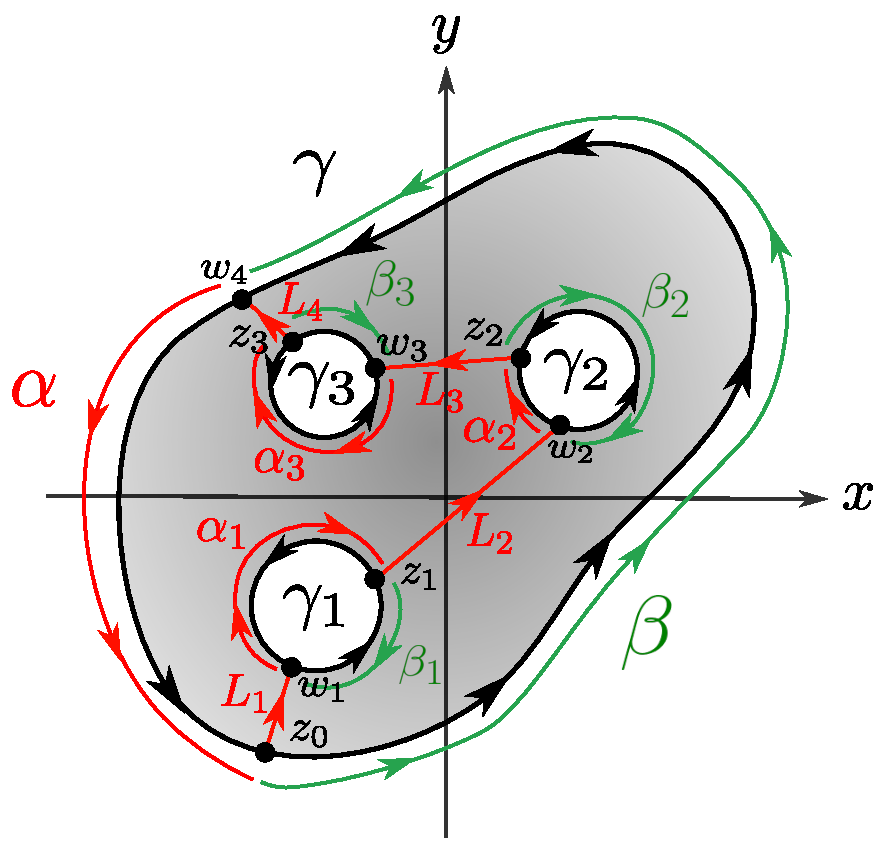
\includegraphics[scale = 0.52]{Figuras/GeneralTCG.pdf}
    \caption{Visión gráfica de la demostración.}
    \label{fig:GeneralTCG}
\end{figure}

Continuamos el proceso hasta encontrar puntos $w_n$ y $z_n$ en $\gamma_n$ y consideramos la curva $\alpha_n$ que parte de $w_n$ hacia $z_n$ siguiendo la curva $\gamma_n$, en sentido contrario. Al final, unimos $z_n$ a un punto $w_{n+1}$ en $\gamma$ mediante un segmento $L_{n+1}$ que no intersecte el camino previo seleccionado de $z_0$ a $z_n$, pasando a través de $w_1, z_1, w_2, z_2, \dots, w_n$. En la selección de estos puntos hemos definido:

\begin{quote}
    La curva $\alpha_j$ que parte del punto $w_j$ hacia $z_j$ siguiendo la curva $\gamma_j$, en sentido contrario, para $j = 1, \dots, n$.
\end{quote}

Ahora definimos:
    
\begin{quote}
  La curva $\beta_j$ como aquella que parte del punto $z_j$ hacia $w_j$ siguiendo la curva $\gamma_j$, en sentido contrario.   
\end{quote}

Ahora, sea $\alpha$ parte de la curva $\gamma$ de $w_{n+1}$ a $z_0$ y sea $\beta$ parte de la curva $\gamma$ de  $z_0$ a $w_{n+1}$, ambas siguiendo el mismo sentido que $\gamma$.

La construcción hecha lleva a dos curvas cerradas $\Gamma_1$ y $\Gamma_2$, ver figura \ref{fig:GeneralTCG}, definidas como sigue:
\begin{align*}
\Gamma_1 &= \alpha + L_1 + \alpha_1 + \cdots + L_{n} + \alpha_n + L_{n+1}, \\
\Gamma_2 &= -L_{n+1} + \beta_n - L_{n} + \cdots + \beta_1 - L_1 + \beta.
\end{align*}

Como $f$ es analítica en $R$, será analítica en los dominios simplemente conexos formados por los interiores de $\Gamma_1$ y $\Gamma_2$. Entonces, por el teorema \ref{CG-SC},
$$\int_{\Gamma_1} f(z) \,dz = 0 ~~\mbox{y}~~ \int_{\Gamma_2} f(z) \,dz = 0.$$

Sumando ambas igualdades, obtenemos que
$$\int_{\Gamma_1} f(z) \,dz  + \int_{\Gamma_2} f(z) \,dz = 0.$$

Dado que
$$\int_{-L_j} f(z) \,dz = - \int_{L_j} f(z)\,dz, \quad j = 1,2, \dots, n+1,$$

concluimos que
$$\int_{\alpha} f(z) \,dz + \int_{\beta} f(z) \,dz + \sum_{j=1}^n \left(\int_{\alpha_j} f(z) \,dz + \int_{\beta_j} f(z) \,dz\right) = 0.$$

Pero,
$$\int_{\alpha_j} f + \int_{\beta_j} f = - \int_{\gamma_j} f ~~\mbox{y}~~ \int_{\alpha} f + \int_{\beta} f = \int_{\gamma} f.$$

Por lo tanto,
$$\int_{\gamma}f(z) \,dz - \sum_{j=1}^n \int_{\gamma_j} f(z) \,dz = 0 \Rightarrow \int_{\gamma} f(z) \,dz= \sum_{j=1}^n \int_{\gamma_j} f(z) \,dz. $$

\end{proof}



\begin{ejemplo}
Sea 
$$f(z) = \frac{1}{z^2(z^2 + 9)}$$

y consideremos el dominio simplemente conexo encerrado por las curvas $\gamma(t) = 2e^{it}$ y $\gamma_1(t) = e^{it}$, $0 \leq t \leq 2\pi$. $f$ es analítica en el interior de $\gamma$ y el exterior de $\gamma_1$. Entonces,
$$\int_{\gamma} \frac{1}{z^2(z^2+9)} = \int_{\gamma_1}\frac{1}{z^2(z^2+9)}.$$
\end{ejemplo}

El ejemplo se puede generalizar al siguiente corolario, el cual es una consecuencia particular del teorema \ref{CGMultiConexo}.

\begin{corolario} \label{CorolarioTCG}
Sean $\gamma_1$ y $\gamma_2$ dos curvas simples cerradas orientadas positivamente, donde $\gamma_2$ es interior a $\gamma_1$ (ver figura \ref{fig:CorlarioTCG}). Si una función $f$ es analítica en la región cerrada que forman esas curvas y los puntos situadas entre ellos, entonces
$$\int_{\gamma_1} f(z) \,dz = \int_{\gamma_2} f(z) \,dz.$$
\end{corolario}

\begin{figure}[H]
    \centering
    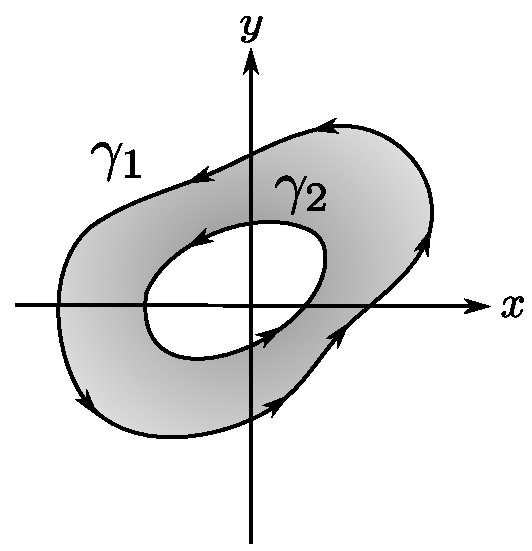
\includegraphics[scale = 0.6]{Figuras/CorolarioTCG.pdf}
    \caption{Principio de deformación de caminos.}
    \label{fig:CorlarioTCG}
\end{figure}

\textbf{Observación:} El corolario se conoce como el \textbf{principio de deformación de caminos}, ya que nos dice que si $\gamma_1$ se deforma continuamente en $\gamma_2$ pasando siempre por puntos en los que $f$ es analítica, el valor de la integral de $f$ sobre $\gamma_1$ no cambia.

\section{Fórmula de Integración de Cauchy}

Según lo calculado en \eqref{PreTIC},
si $\gamma$ es la circunferencia unitaria $\gamma(t) = e^{it}, 0 \leq t \leq 2\pi$, tenemos que
$$\int_{\gamma} \frac{1}{z} \,dz = 2\pi i$$

o, equivalentemente,
$$1 = \frac{1}{2\pi i} \int_{\gamma} \frac{1}{z} \,dz. $$

Notemos que $\gamma$ es cerrada e inyectiva en el intervalo $[0,2\pi[$. 

Ahora, consideremos una nueva curva $\alpha(t) = e^{it}, 0\leq t \leq 4\pi$ y repitamos el cálculo anterior
$$\int_{\alpha} \frac{1}{z} \,dz = \int_0^{4\pi} \frac{1}{e^{it}} i e^{it} \,dt = \int_0^{4\pi} i dt = 4\pi i,$$

es decir,
$$2 = \frac{1}{2\pi i} \int_{\alpha} \frac{1}{z} \,dz.$$

De forma inductiva, si $n \in \mathbb{N}$, entonces
$$n = \frac{1}{2\pi i} \int_{\gamma_n} \frac{1}{z} \,dz,$$

donde $\gamma_n(t) = e^{it}, 0 \leq t \leq 2n\pi.$

Finalmente, si $\tilde{\gamma}$ es otra curva cerrada, que envuelve al origen y que puede deformarse en alguna $\gamma_n$, ésto es, se puede aplicar el corolario \ref{CorolarioTCG}. Entonces,
$$n = \frac{1}{2\pi i} \int_{\gamma_n} \frac{1}{z} \,dz =  \frac{1}{2\pi i} \int_{\tilde{\gamma}} \frac{1}{z} \,dz.$$

Notemos que este número $n$ indica las veces que gira la curva en torno del origen y éste será positivo si gira contrario a las agujas del reloj y será negativo en el otro caso (segundo postulado del teorema \eqref{PropiedadesILinea}).

En general, para cualquier punto $z_0 \in \mathbb{C}$, se ve que el número de veces que una curva cerrada $\tilde{\gamma}$ gira alrededor de $z_0$ es
$$n = \frac{1}{2\pi i} \int_{\tilde{\gamma}}\frac{1}{z-z_0} \,dz$$

por un argumento similar. Observemos que si $z_0$ está al exterior de $\gamma$, entonces
$$0 = \frac{1}{2\pi i} \int_{\gamma} \frac{1}{z-z_0} \,dz.$$

Esta idea conduce a formular la siguiente definición.

\begin{defi}
Sea $\gamma$ una curva cerrada que envuelve al punto $z_0 \in \mathbb{C}$. Llamaremos \textbf{índice de $\gamma$} al número
$$I(\gamma,z_0) = \frac{1}{2\pi i} \int_{\gamma} \frac{1}{z-z_0} \,dz \in \mathbb{Z}.$$
\end{defi}

\begin{teorema}[Fórmula integral de Cauchy] \label{FIC}
Sea $f$ una función analítica en una región simplemente conexa $D$ y sea $\gamma$ una curva cerrada en $D$. Entonces, para cualquier $z_0 \in D$,
$$f(z_0) I(\gamma,z_0) = \frac{1}{2\pi i} \int_{\gamma} \frac{f(z)}{z-z_0} \,dz.$$
\end{teorema}

\begin{proof}
Se define
$$g(z) = \left\{ \begin{array}{cl}
    \frac{f(z) - f(z_0)}{z-z_0}, & \mbox{si} ~ z \neq z_0  \\
    f'(z_0), & \mbox{si} ~ z = z_0
\end{array} \right. .$$

Claramente, $g$ es analítica para todos los $z \neq z_0$ y $\lim\limits_{z \to z_0} g(z) = f'(z_0)$, pues $f$ es analítica. Consideremos $\gamma_{\varepsilon}(t) = z_0 + \varepsilon e^{it}; 0 \leq t \leq 2\pi m$, con $\varepsilon > 0$ tal que $\gamma_{\varepsilon}$ esté al interior de $\gamma$. Por el teorema de Cauchy-Goursat para regiones múltiplemente conexas,
$$\int_{\gamma} g(z) \,dz = \int_{\gamma_{\varepsilon}} g.$$

Por otro lado, $g$ es acotada cerca de $z_0$ (pues $g$ es continua en $z_0$), entonces existe $M > 0$ tal que $|g(z)| \leq M$ para $|z-z_0| < r_0$ con $r_0 > 0$ pequeño. Luego,
$$\left| \int_{\gamma} g(z) \,dz \right| = \left| \int_{\gamma_{\varepsilon}} g(z) \,dz \right| \leq M l(\gamma_{\varepsilon}) = M 2\pi \varepsilon. $$

Como $\varepsilon >0$ es arbitrario, se concluye que
$$\int_{\gamma} g(z) \,dz = 0. $$

Finalmente,
\begin{align*}
    0 = \int_{\gamma} g(z) \,dz &= \int_{\gamma} \frac{f(z)}{z-z_0} \,dz - \int_{\gamma} \frac{f(z_0)}{z-z_0} \,dz \\
    &=  \int_{\gamma} \frac{f(z)}{z-z_0} \,dz - f(z_0) \int_{\gamma} \frac{1}{z-z_0} \,dz \\
    &=  \int_{\gamma} \frac{f(z)}{z-z_0} \,dz - f(z_0) I(\gamma,z_0) 2\pi i.
\end{align*}

Despejando, se tiene
$$f(z_0) I(\gamma,z_0) = \frac{1}{2\pi i} \int_{\gamma} \frac{f(z)}{z-z_0} \,dz.$$
\end{proof}

\begin{corolario}
Sea $f$ una función analítica en una región simplemente conexa $D$ y sea $\gamma$ una curva simple cerrada en $D$, orientada positivamente. Entonces, para cualquier punto $z_0$ en el interior de $\gamma$, se tiene
$$f(z_0) = \frac{1}{2\pi i} \int_{\gamma} \frac{f(z)}{z-z_0} \,dz.$$
\end{corolario}

\begin{ejemplo}
Sea $C$ el contorno del cuadrado cuyos lados están sobre las rectas $x = \pm 2$ e $y = \pm 2$, con $C$ recorrido positivamente. Calcular
$$\int_C \frac{\cos(z)}{z(z^2+8)} \,dz.$$

\textbf{Solución:} Notemos que podemos escribir 
$$\frac{\cos(z)}{z(z^2+8)} = \frac{\cos(z)}{z(z + 2\sqrt{2}i)(z- 2\sqrt{2}i)}.$$

Claramente el denominador se anula en $z = 0, \pm 2\sqrt{2}i$, pero sólo el punto $z = 0$ está dentro del cuadrado $C$. Entonces, si hacemos $f(z) =  \cos(z)/(z^2+8)$, $f$ es analítica en el interior del cuadrado (región simplemente conexa). Entonces, por el teorema de la fórmula integral de Cauchy,
$$\int_C \frac{\cos(z)}{z(z^2+8)} \,dz = \int_C \frac{f(z)}{z} \,dz = 2\pi i f(0) = \frac{2\pi i}{8} = \frac{\pi i}{4}.  $$
\end{ejemplo}

\subsection{Derivadas bajo el signo de la integral*}

Nos centraremos en la analiticidad de una función de la forma
$$g(z) = \int_{\gamma} \phi(z,\xi) \,d\xi,$$

donde $\xi$ yace en la curva simple cerrada $\gamma$ y $z$ pertenece a un conjunto abierto. 

\begin{lema} \label{LemaDerivadaIntegral}
Supongamos que $f$ es analítica en un conjunto abierto que contiene a la bola cerrada $\Bar{B}(z_0,R) = \{ z \in \mathbb{C}: d(z,z_0) \leq R\}$ y satisface $|f(z)| \leq M$ para todo $z \in \Bar{B}(z_0,R)$. Entonces, para $0 < |z-z_0| < \frac{R}{2}$ es válido:
\begin{equation}
\left| \frac{f(z) - f(z_0)}{z-z_0}  - f'(z_0)\right| \leq 2M \frac{|z-z_0|}{R^2}    \label{DerivadaIntegral1}
\end{equation}

y

\begin{equation}
   f'(z_0) = \frac{1}{2\pi i} \int_{C(z_0,R)} \frac{f(\xi)}{(\xi - z_0)^2} \,d\xi, \label{DerivadaIntegral2}
\end{equation}
    
donde $C(z_0,R) = Fr(\Bar{B}(z_0,R))$.
\end{lema}

\begin{proof}
Usando \ref{FIC} para $0 < |z-z_0| < \frac{R}{2}$,  escribimos
$$f(z) = \frac{1}{2\pi i} \int_{C(z_0,R)} \frac{f(\xi)}{\xi-z}d \xi ~~\mbox{y}~~ f(z_0) = \frac{1}{2\pi i} \int_{C(z_0,R)} \frac{f(\xi)}{\xi-z_0}d \xi.$$

Combinando estas integrales y simplificando, obtenemos
\begin{equation}
 \frac{f(z) - f(z_0)}{z-z_0} = \frac{1}{2\pi i}   \int_{C(z_0,R)} \frac{f(\xi)}{(\xi-z)(\xi - z_0)} d\xi. \label{DemDerivadaIntegral1}
\end{equation}

Para $\xi \in C(z_0,R)$ y $0 < |z-z_0| < \frac{R}{2}$, tenemos que
$$||\xi - z_0| - |z-z_0||\leq |(\xi-z_0) - (z-z_0) | =  |\xi - z| \Rightarrow |\xi - z_0| \leq |\xi -z| + |z-z_0|.$$

Como $|\xi - z_0| = R$, pues $\xi \in C(z_0,R)$, concluimos que
$$R \leq |\xi-z| + \frac{R}{2} \Rightarrow |\xi - z| \geq \frac{R}{2} \Rightarrow \frac{1}{|\xi - z|} \leq \frac{2}{R}.$$

Por lo tanto, 
$$\left| \frac{f(\xi)}{(\xi-z)(\xi-z_0)} - \frac{f(\xi)}{(\xi-z_0)^2} \right| = \left| \frac{f(\xi)(z-z_0)}{(\xi-z)(\xi-z_0)^2} \right| \leq M \frac{2}{R} \frac{|z-z_0|}{R^2} = 2M \frac{|z-z_0|}{R^3}.$$

Usando el teorema \ref{CotaIntegral}, se tiene que 
$$\left| \frac{1}{2\pi i} \int_{C(z_0,R)}\left[  \frac{f(\xi)}{(\xi-z)(\xi-z_0)} - \frac{f(\xi)}{(\xi-z_0)^2}\right] \,d\xi \right| \leq \frac{2\pi R}{|2\pi i|} \frac{2M|z-z_0|}{R^3} = 2M \frac{|z-z_0|}{R^2}.$$

Separando las integrales y haciendo uso de la ecuación \eqref{DemDerivadaIntegral1}, obtenemos
\begin{equation}
 \left| \frac{f(z)-f(z_0)}{z-z_0} - \frac{1}{2\pi i}\int_{C(z_0,R)} \frac{f(\xi)}{(\xi-z_0)^2} \,d\xi \right|  \leq 2M \frac{|z-z_0|}{R^2}. \label{DemDerivadaIntegral2}
\end{equation}

Haciendo $z \to z_0$ en \eqref{DemDerivadaIntegral2} deducimos que 
$$f'(z_0) = \frac{1}{2\pi i} \int_{C(z_0,R)} \frac{f(\xi)}{(\xi - z_0)^2} \,d\xi.$$

Reemplazando en \eqref{DemDerivadaIntegral2}, obtenemos \eqref{DemDerivadaIntegral1}.
\end{proof}

\begin{teorema} \label{TeoDerivadaIntegral}
Sea $\gamma$ una curva y $A$ un conjunto abierto. Sea $\phi(z,\xi)$ una función definida para $z \in A$ y $\xi$ en $\gamma$. Supongamos que $\phi(z,\xi)$ es continua en $\xi$ pertenecientes a $\gamma$ y analítica en $z\in A$ y que la derivada compleja $\frac{d\phi}{dz}(z,\xi)$ es continua para $\xi$ en $\gamma$. Entonces, la función
\begin{equation}
g(z) = \int_{\gamma} \phi(z,\xi) \,d\xi    \label{DerivadaIntegral3}
\end{equation}

es analítica en $A$ y su derivada es
\begin{equation}
g'(z) = \int_{\gamma} \frac{d\phi}{dz}(z,\xi) \,d\xi.    \label{DerivadaIntegral4}
\end{equation}

\end{teorema}

\begin{proof}
Fijemos un punto $z_0 \in A$ y elijamos $R > 0$ tal que $\Bar{B}(z_0,R)$ esté contenida en $A$. Sea 
$$M = \max_{z \in \overline{B}(z_0,R), \xi \in C} |\phi(z,\xi)|,$$

el cual es finito porque la función es continua en un conjunto compacto. 

Como $\phi(z,\xi)$ es una función analítica con respecto a $z$ en $A$. Para cada $z$ tal que $0 < |z-z_0| < \frac{R}{2}$ y $\xi$ en $\gamma$, el lema \ref{LemaDerivadaIntegral} implica que
\begin{equation}
\left| \frac{\phi(z,\xi) - \phi(z_0,\xi)}{z-z_0} - \frac{d\phi}{dz}(z_0,\xi) \right| \leq 2M \frac{|z-z_0|}{R^2}.    \label{DemDerivadaIntegral3}
\end{equation}

Integrando la expresión dentro del valor absoluto al lado derecho en \eqref{DemDerivadaIntegral3} y usando \eqref{DerivadaIntegral3}, encontramos que
\begin{align}
    \left| \frac{g(z)-g(z_0)}{z-z_0} - \int_{\gamma} \frac{d\phi}{dz}(z_0,\xi) \,d\xi \right| &= \left| \frac{\int_{\gamma} [\phi(z,\xi) - \phi(z_0,\xi)] \,d\xi}{z-z_0} - \int_{\gamma} \frac{d\phi}{dz}(z_0,\xi) \,d\xi \right| \nonumber \\
    &= \left| \int_{\gamma} \left[ \frac{\phi(z,\xi) - \phi(z_0,\xi)}{z-z_0} - \frac{d\phi}{dz}(z_0,\xi) \right] \,d\xi  \right|  \nonumber \\
    &\leq l(\gamma) 2M \frac{|z-z_0|}{R^2}. \label{DemDerivadaIntegral5}
\end{align}

Por lo tanto, haciendo $z \to z_0$ en \eqref{DemDerivadaIntegral5} deducimos que 
$$g'(z_0) =  \int_{\gamma} \frac{d\phi}{dz}(z,\xi) \,d\xi.$$
\end{proof}

\subsection{Fórmula de la integral de Cauchy generalizada }

Ahora estamos preparados para probar que si una función es analítica en un punto, admite derivadas de todos los órdenes en ese punto, y todas ellas son analíticas en él.

\begin{teorema} \label{GeneralFIC}
Sea $f$ una función analítica en una región $D$. Entonces, $f$ admite derivadas de todos los órdenes en $D$; más aún, si $z_0 \in D$ y $\gamma$ es una curva cerrada en $D$, tal que su interior sigue estando en $D$, para la que $z_0$ no está en $\gamma$, entonces
\begin{equation}
f^{(k)}(z_0) I(\gamma,z_0) =  \frac{k!}{2\pi i} \int_{\gamma} \frac{f(z)}{(z-z_0)^{k+1}} \,dz.    \label{FICDerivadas}
\end{equation}

\end{teorema}

\begin{proof}
Sin pérdida de generalidad, podemos asumir que $I(\gamma,z_0) = 1$, es decir, $z_0$ está en el interior de $\gamma$ y la curva es simple orientada positivamente. Demostraremos el teorema por inducción matemática (partiendo del $n = 0$). 

Cuando $n = 0$, $f^{(0)}(z) = f(z)$ y $0! = 1$, en este caso la identidad fue probada en el teorema \ref{FIC}. Sea $A$ el interior de la curva $\gamma$. Asumiendo por inducción que \eqref{FICDerivadas} es válida para cualquier $n \in \mathbb{N}$; para $z \in A$ y $\xi$ en $\gamma$, definimos:
$$\phi(z,\xi) = \frac{n!}{2\pi i} \frac{f(\xi)}{(\xi-z)^{n+1}},$$

tal que
$$f^{(n)}(z) = \int_{\gamma} \phi(z,\xi) \,dz.$$

Notemos que $\phi(z,\xi)$ es analítica en la variable $z$ en $A$ y continua para $\xi$ en $\gamma$. Más aún, 
$$\forall z \in A: ~ \frac{d\phi}{dz}(z,\xi) = \frac{(n+1)!}{2\pi i} \frac{f(\xi)}{(\xi - z)^{n+2}},$$

la cual es continua para $\xi$ en $\gamma$. Usando el teorema \ref{TeoDerivadaIntegral}, obtenemos que $f^{(n+1)}$ es analítica en $A$ y
$$\forall z \in A: ~ f^{(n+1)}(z) = \frac{(n+1)!}{2\pi i} \int_{\gamma} \frac{f(\xi)}{(\xi-z)^{n+2}} \,d\xi.$$
\end{proof}

\begin{ejemplo}
Sea $\Gamma$ la curva que se ilustra en la figura \ref{fig:EjemploFIC}. Determinar
    $$\int_{\Gamma} \frac{z}{(z-i)(z^2+1)} \,dz.$$
    
\textbf{Solución:}  Notemos que podemos escribir
$$ \frac{z}{(z-i)(z^2+1)} = \frac{z}{(z-i)^2(z+i)}.$$

El denominador se anula en $z = \pm i$ y ambos puntos están en el interior de la curva $\Gamma$, entonces la descomponemos en dos curvas $\Gamma_1$ y $\Gamma_2$, como se visualiza en la figura \ref{fig:EjemploFIC}.
\begin{figure}[H]
    \centering
    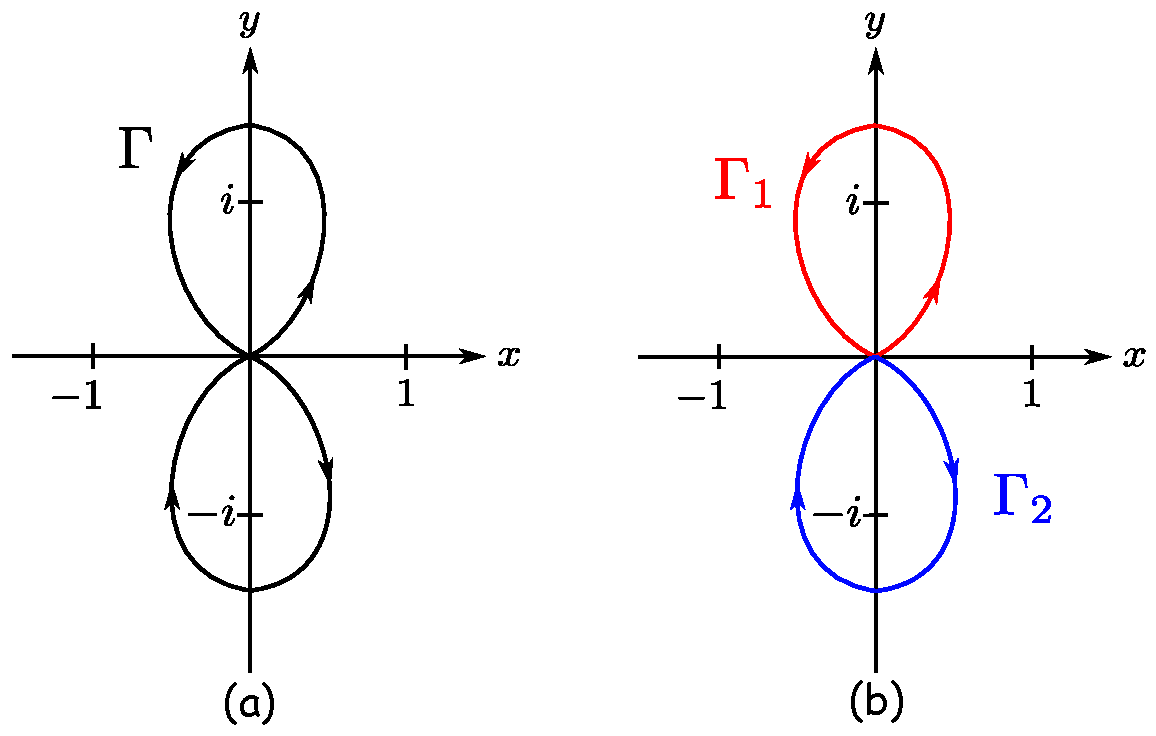
\includegraphics[scale = 0.5]{Figuras/Ejemplo_FIC.pdf}
    \caption{Curva ocho $\Gamma$ en (a) dividida en dos curvas $\Gamma_1$ y $\Gamma_2$ en (b).}
    \label{fig:EjemploFIC}
\end{figure}

Así, 
$$\int_{\Gamma} \frac{z}{(z-i)(z^2+1)} \,dz = \int_{\Gamma_1} \frac{z}{(z-i)(z^2+1)} \,dz + \int_{\Gamma_2} \frac{z}{(z-i)(z^2+1)} \,dz.$$

Ahora podremos usar la fórmula de la integral de Cauchy. Observe que la orientación de las nuevas curvas son distintos: La orientación de $\Gamma_1$ es positiva, mientras que la orientación de $\Gamma_2$ es negativa. Para $\Gamma_1$, aplicamos \ref{FICDerivadas} con $n = 1$, $f(z) = \frac{z}{z+i}$ y $z_0 =i$:
$$\int_{\Gamma_1} \frac{f(z)}{(z-i)^2} \,dz = 2\pi i \frac{d}{dz}\left[ \frac{z}{z+i} \right]_{z=i} = \left. 2\pi i \frac{i}{(z+i)^2} \right|_{z=i} = \frac{\pi}{2}.$$

Para $\Gamma_2$,  aplicamos \ref{FICDerivadas} con $n = 0$, $f(z) = \frac{z}{(z-i)^2}$ y $z_0 = -i$, teniendo en cuenta la orientación de $\Gamma_2$,
$$\int_{\Gamma_2} \frac{f(z)}{z+i} \,dz = \left. - 2\pi i  \frac{z}{(z-i)^2} \right|_{z=-i} = \frac{\pi}{2}.$$

Por lo tanto,
$$\int_{\Gamma} \frac{z}{(z-i)(z^2+1)} \,dz = \pi.$$
\end{ejemplo}

\begin{corolario}\label{corolarioFIC}
Supongamos que $f$ es analítica en un abierto $A$. Entonces $f$ tiene derivadas de todos los órdenes $f',f'',f^{(3)}, f^{(4)},\dots$ las cuales son funciones analíticas en $A$.
\end{corolario}

\begin{proof}
Para $z \in A$, sea $\overline{B}(z,R)$ la bola cerrada contenida en $A$ y $C$ su frontera. Por el teorema \ref{GeneralFIC}, todas las derivadas de $f$ existen en $A\setminus C$, y en particular en el punto $z$ dado.
\end{proof}

\textbf{Observación:} Consideremos la función real $f(x) = x^{5/3}, - \infty < x < \infty$. Sus derivada, $f'(x) = \frac{5}{3} x^{2/3}$, existe y es continua para todo $x \in \mathbb{R}$; sin embargo, $f''(x)$ no existe en $x = 0$. Por lo tanto, este corolario no tiene un análogo para el caso real.

\subsection{Teorema de Morera}

El siguiente teorema es un recíproco parcial del teorema de Cauchy.

\begin{teorema}[de Morera]
Sea $f$ continua en una región $D$ (abierto conexo) y suponga que 
$$\int_{\gamma} f(z) \,dz = 0,$$

para cualquier curva cerrada en $D$. Entonces, $f$ es analítica en $D$, y $f = F\,'$ para alguna función analítica $F$ en $D$.
\end{teorema}

\begin{proof}
De acuerdo al teorema \ref{TFC2}, $f$ admite una primitiva en $D$, es decir, existe una función analítica $F$ tal que $F'(z) = f(z)$ en todo punto de $D$. 

Ahora, de \ref{corolarioFIC}, la derivada de una función analítica es también analítica; y puesto que $f$ es la derivada de $F$, se sigue que $f$ es analítica en $D$.

\end{proof}

\textbf{Observación:} En particular, cuando $D$ es simplemente conexo, tenemos, para la clase de las funciones continuas en $D$, un recíproco del teorema de Cauchy-Goursat para tales dominios.

\section{Módulo máximo}

\subsection{Teorema del módulo máximo}

Partamos con los siguientes ejercicios:

\begin{ejemplo} \label{EjemploTVM}
\ 

\begin{enumerate}
    \item Si $f$ y $\overline{f}$ son analíticas en $D$, entonces $f$ es constante. 
    
    En efecto, sea $f(z) = u(x,y) + iv(x,y)$, entonces $\overline{f(z)} = u(x,y) - iv(x,y)$. Por la condición de ser funciones analíticas, se tiene que se satisfacen las ecuaciones de Cauchy-Riemann, es decir, 
    $$u_x = v_y, \quad u_y = -v_x; \quad u_x = -v_y, \quad u_y = v_x,$$
    
    respectivamente. De aquí, se tiene que las derivadas parciales de $u$ y $v$ son iguales a 0 y, por tanto, constantes.
    
    \item Si $|f(z)| = C$, con $C$ una constante distinta de cero, para todo $z \in D$, y $f$ es analítica, entonces $f = cte$ en $D$.
    
    En efecto, notemos que 
    $$C^2 = |f(z)|^2 = f(z) \overline{f(z)}.$$
    
    Como $f(z) \neq 0$ para todo $z \in D$, se tiene que 
    $$\forall z\in D: ~ \overline{f(z)} = \frac{C^2}{f(z)},$$
    
    la cual analítica. Por lo demostrado en el ejercicio anterior, $f$ es constante en $D$.
\end{enumerate}
\end{ejemplo}

Si $f$ es analítica y no es constante en una región abierta que contiene al disco $|z-z_0| < r_0$ y continua en $|z-z_0| \leq r_0$, entonces, al ser compacto, el módulo de $f$ alcanza su máximo en $|z-z_0| \leq r_0$, pero ¿en qué lugar del disco cerrado alcanza ese máximo y en que lugar no?

\begin{lema} \label{LemaModuloMaximo}
Sea $f$ analítica en un entorno $|z-z_0| < r_0$ de un punto $z_0$. Si $|f(z)| \leq |f(z_0)|$ para todo $z$ de ese entorno, entonces $f(z)$ tiene valor constante $f(z_0)$ sobre ese entorno.
\end{lema}

\begin{proof}
Supongamos que $f$ es analítica en dicho entorno. Sea $z_1$ cualquier punto del entorno distinto del $z_0$, y sea $r = d(z_1,z_0)$. Si consideramos la circunferencia $\gamma(t) = z_0 + re^{it}, 0 \leq t \leq 2\pi$, la fórmula integral de Cauchy nos dice que 
$$f(z_0) = \frac{1}{2\pi} \int_{\gamma} \frac{f(z)}{z-z_0} \,dz.$$

Usando la representación paramétrica de la curva, tenemos
$$
f(z_0) = \frac{1}{2\pi i} \int_0^{2\pi} \frac{f\left(z_0 +  re^{it}\right)}{(z_0 +  re^{it}) - z_0} i r e^{it} \,dt = \frac{1}{2\pi} \int_0^{2\pi} f(z_0 +  re^{it})\,dt.   
$$

Luego,
\begin{equation}
|f(z_0)| \leq \frac{1}{2\pi} \int_0^{2\pi} \left|f\left(z_0 +  re^{it}\right) \right| \,dt.    \label{TVM1}
\end{equation}

Por hipótesis, sabemos que $|f(z)| \leq |f(z_0)|$, para $|z-z_0| < r_0$, entonces
\begin{align}
 \frac{1}{2\pi} \int_0^{2\pi} \left|f\left(z_0 +  re^{it}\right) \right| \,dt &\leq   \frac{1}{2\pi} \int_0^{2\pi} |f(z_0)|\,dt \nonumber \\
 &= \frac{1}{2\pi} |f(z_0)| 2\pi = |f(z_0)|. \label{TVM2}
\end{align}

Combinando \eqref{TVM1} y \eqref{TVM2}, se tiene que 
\begin{align*}
   \frac{1}{2\pi} \int_0^{2\pi} & \left|f\left(z_0 +  re^{it}\right) \right| \,dt \leq |f(z_0)| \leq \frac{1}{2\pi} \int_0^{2\pi} \left|f\left(z_0 +  re^{it}\right) \right| \,dt \\
  &\Rightarrow |f(z_0)| = \frac{1}{2\pi} \int_0^{2\pi} \left|f\left(z_0 +  re^{it}\right) \right| \,dt \\
   &\Leftrightarrow \int_0^{2\pi} \left[ \left| f(z_0 + re^{it}) \right| - |f(z_0)|\right] \,dt = 0. 
\end{align*}

Por la continuidad de la función integrada, tenemos que 
$$|f(z_0 + re^{it})| = |f(z_0)|, \quad 0 \leq t \leq 2\pi.$$

Esto demuestra que $|f(z)| = |f(z_0)|$ para todo $z$ en la circunferencia $|z-z_0| = r$.

Finalmente, al ser $z_1$ un punto arbitrario del entorno, $0 <r <r_0$ también lo es, por tanto $|f(z)| = |f(z_0)|$ sobre el entorno $0 < |z-z_0| < r_0$. Pero sabemos, por el ejemplo \ref{EjemploTVM}, que cuando el módulo de una función analítica es constante en un dominio, la propia función es constante en él. Luego $f(z) = f(z_0)$ en todo punto del entorno.
\end{proof}

\begin{teorema}[del módulo máximo]
Si $f$ es analítica en una región abierta conexa $D$ y existe $z_0 \in D$ tal que $|f(z)| \leq |f(z_0)|$ para todo $z \in D$, entonces $f$ es constante en $D$.
\end{teorema}

\begin{proof}
Probaremos que $|f|$ es constante en $D$, para así concluir que $f$ es constante.

Sea $w \in D$ cualquiera. Como $D$ es conexo, existe un camino poligonal que conecta $z_0$ a $w$, ver figura \ref{fig:ModuloMaximo}. El camino está constituido por una secuencia finita de puntos, en particular, $z_0,z_1, \dots, z_n = w$, pero $D$ es abierto, así que tenemos también una secuencia de bolas abiertas $\{B_0, B_1, \dots, B_n\}$ que satisfacen:
\begin{enumerate}
    \item $B_i$ está contenida en $D$ para $i = 1,2, \dots,n$.
    
    \item $B_i$ contiene al punto $z_{i+1}$ para $i = 0,1, \dots, n-1$.
\end{enumerate}

\begin{figure}[H]
    \centering
    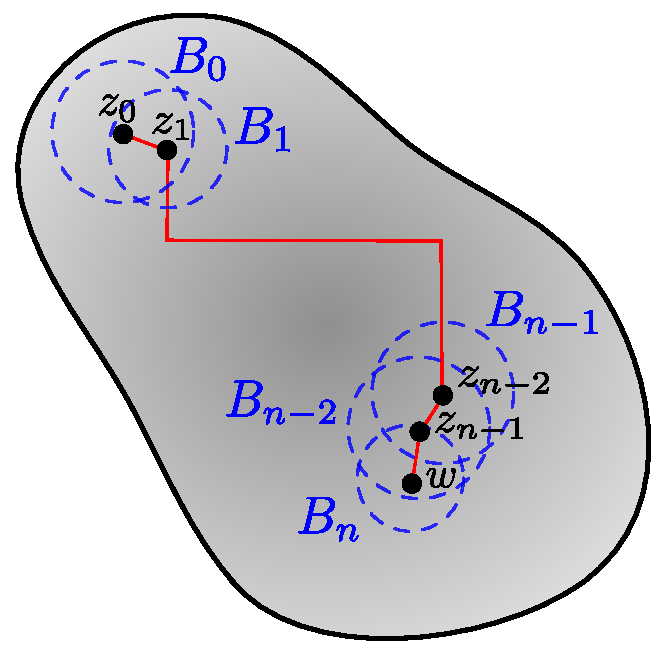
\includegraphics[scale = 0.53]{Figuras/ModuloMaximo.pdf}
    \caption{Demostración del teorema del módulo máximo.}
    \label{fig:ModuloMaximo}
\end{figure}

Debido a que $|f(z)| \leq |f(z_0)|$ para todo $z \in D$,  es el máximo valor de $|f(z)|$ para los $z \in B_0$. Por el lema \ref{LemaModuloMaximo}, $|f(z)|$ es contante en $B_0$. En particular, $|f(z_0)| = |f(z_1)|$, pues $z_1 \in B_0$. Entonces, $|f(z_1)|$ es el máximo valor de $|f(z)|$ en $B_1$. De nuevo, por el lema \ref{LemaModuloMaximo}, $|f(z)|$ es contante en $B_1$. Usando el mismo argumento repetidamente, deducimos que $|f(z)|$ es constante sobre las bolas abiertas $B_0, B_1, \dots, B_n$. En particular, $|f(z_0)| = |f(w)|$. Ahora, como $w$ es arbitrario, concluimos que $|f|$ es constante en $D$. Por lo tanto, $f$ es constante en $D$.  
\end{proof}

El siguiente corolario es consecuencia directa del teorema del módulo máximo y es directamente aplicable a problemas de búsqueda de máximos.

\begin{corolario}
Sea $f$ una función analítica y no constante en una región $D$ y sea $\gamma$ una curva simple cerrada enteramente contenida en $D$. Entonces, el máximo valor alcanzado por $|f(z)|$ en el compacto encerrado por la curva $\gamma$ se alcanza en, precisamente,  $\gamma$.
\end{corolario}

\begin{ejemplo}
Determinar el máximo absoluto de $|f(z)|$ en $|z| \leq 1$ para la función $f(z) = z^2 -3z+2$.
\\

\textbf{Solución:} La función es no constante, analítica en $|z| < 1$ y continua en $|z| = 1$, el teorema del módulo máximo nos dice que el máximo valor de $|f(z)|$ se alcanza en $|z| = 1$. Haciendo $z = x+iy$, tenemos
$$f(z) = f(x+iy) = (x^2 - y^2 -3x+2) + i(2xy-3y).$$

Maximicemos
$$|f(z)|^2 = (x^2 - y^2 -3x+2)^2 + (2xy-3y)^2$$

con la condición $|z| = x^2+y^2 = 1$. Para ello, despejando $y$, $y^2 = 1-x^2$:
\begin{align*}
    |f(z)|^2 &= (2x^2 -3x+1)^2 + (1-x^2)(2x-3)^2 \\
    &= 8x^2 -18x+10, \quad x \in [-1,1].
\end{align*}

Queda como ejercicio para el lector verificar, por medio del teorema de los valores extremos, que el máximo absoluto de $g(x) = 8x^2 -18x+10 $ en $[-1,1]$ es $g(-1) = 36$. Por lo tanto, el máximo módulo de $f$ es
$$|f(-1)| = \sqrt{36} = 6.$$
\end{ejemplo}

\subsection{Teorema de Liouville y el teorema fundamental del Álgebra} 

Dos importantes consecuencias del teorema del módulo máximo son los siguientes teoremas.

\begin{teorema}[de Liouville]
Si $f$ es una función entera y acotada, entonces $f$ es constante.
\end{teorema}

\begin{proof}
Por las hipótesis, existe $M > 0$ tal que
$$\forall z \in \mathbb{C}: ~ |f(z)| \leq M.$$

Luego, para cualquier $z_0 \in \mathbb{C}$ y la circunferencia $C_r: |z-z_0| = r$, se tiene
\begin{align*}
    |f'(z_0)| = \left|\frac{1}{2\pi i} \int_{C_r} \frac{f(z)}{(z-z_0)^2} \,dz \right| &\leq \frac{1}{2\pi} \int_{C_r} \frac{|f(z)|}{|z-z_0|^2} \,|dz| \\
    &\leq \frac{M}{2\pi r^2} \int_{C_r} |dz| \\
    &= \frac{M}{2\pi r^2} 2\pi r = \frac{M}{r}.
\end{align*}

Como $r$ es arbitrario, se concluye que $f'(z_0) = 0$. Pero $z_0$ es, también, arbitario, por tanto
$$f'(z) = 0 \Rightarrow f = cte.$$
\end{proof}

\begin{teorema}[Fundamental del Álgebra]
Cualquier polinomio 
$$P(z) = a_0 + a_1 z + a_2 z^2 + \cdots + a_n z^n,$$

con $a_n \neq 0$ y $n\geq 1$, tiene, al menos, una raíz. Ésto es, existe $z_0 \in \mathbb{C}$ tal que $P(z_0) = 0$.
\end{teorema}

\begin{proof}
Si suponemos que no existe tal raíz, entonces la función
$$f(z) = \frac{1}{P(z)}$$

es una función entera. Mostremos que $f$ es acotada o, equivalentemente, $P$ es acotado.

Notemos que, para cualquier $|z|> 1$, se tiene
\begin{align*}
    |P(z)| &= |z|^{n-1} \left| a_n z + \frac{a_{n-1}}{1} + \frac{a_{n-2}}{z} + \cdots + \frac{a_0}{z^{n-1}} \right| \\
    &\geq |z|^{n-1} \left[ |a_n z|- \frac{|a_{n-1}|}{1} - \frac{|a_{n-2}|}{|z|} - \cdots - \frac{|a_0|}{|z^{n-1}|} \right]
\end{align*}

y si llamamos $a = |a_{n-1}| + \cdots + |a_0|$, entonces
\begin{align*}
  |P(z)|  &\geq |z|^{n-1} \left[ |a_n z|- \frac{|a_{n-1}|}{1} - \frac{|a_{n-2}|}{|z|} - \cdots - \frac{|a_0|}{|z^{n-1}|} \right]  \\
  &\geq |z|^{n-1} \left[ |a_n|\,|z| - |a_{n-1}| - |a_{n-2}| - \cdots - |a_0| \right] \\
  &= |z|^{n-1} \left[ |a_n|\,|z| -a \right].
\end{align*}

Sea $M > 0$ dado y consideremos $K = \max\left\{1, \frac{M+a}{|a_n|} \right\}$, luego para $|z| > K$, se tiene que
$$|P(z)| \geq  |z|^{n-1} \left[ |a_n|\,|z| -a \right] >  \left[ |a_n|\, \frac{M+a}{|a_n|} -a \right] = M $$

de donde se concluye que
$$|z| > K \Rightarrow |f(z)| = \frac{1}{|P(z)|} < \frac{1}{M}.$$

Ahora, $f$ es continua en la bola cerrada de centro $0$ y radio $K$, luego $f$ es acotada aquí por algún $N > 0$. Así,
$$\forall z \in \mathbb{C}: ~ |f(z)| \leq \max\left\{ N,\frac{1}{M} \right\}.$$

Por el teorema de Liouville, $f$ es constante, lo que implica que $P$ es constante. Ésto es una contradicción, ya que del hecho que $a_n \neq 0$, $P$ no es constante. Tal contradicción viene de suponer que $f(z) \neq 0$, para todo $z \in \mathbb{C}$. De esta manera, hemos probado que existe $z_0 \in \mathbb{C}$ tal que
$$f(z_0) = 0.$$
\end{proof}

